\chapter{Mikroprozessoren II}

Zusammenfassung der Vorlesung "`Mikroprozessoren II"' aus dem Wintersemester 2015.\footnote{\url{https://capp.itec.kit.edu/teaching/mp2/?lang=d&sem=ws15}}

\section{Einführung}

Entwurf einer Rechneranlage: Ingenieurmäßige Aufgabe der Kompromissfindung zwischen:
\begin{itemize}
	\item Zielsetzung: Einsatzgebiet, Anwendungsbereich, Leistung, Verfügbarkeit, etc.
	\item Randbedingungen: Technologie, Größe, Geld, Energieverbrauch Umwelt, etc.
	\item Gestaltungsgrundsätze: Modularität, Sparsamkeit, Fehlertoleranz, etc.
	\item Anforderungen: Kompatibilität, Betriebssystemanforderungen, Standards, etc.
\end{itemize}


\subsection{Entwurfsfragen: Zielsetzungen}

\subsubsection{Einsatzgebiete}
\begin{itemize}
	\item \textbf{Desktop Computing}
	\begin{itemize}
		\item PCs bis Workstations (\$1000 - \$10.000)
		\item Günstiges Preis-/Leistungsverhältnis
		\item Ausgewogene Rechenleistung für ein breites Spektrum von (interaktiven) Anwendungen
	\end{itemize}
	\item \textbf{Server}
	\begin{itemize}
		\item Rechen- und datenintensive Anwendungen
		\item Hohe Anforderungen an die Verfügbarkeit und Zuverlässigkeit
		\item Skalierbarkeit
		\item Große Dateisysteme und Ein-/Ausgabesysteme
	\end{itemize}
	\item \textbf{Eingebettete Systeme}
	\begin{itemize}
		\item Mikroprozessorsysteme, eingebettet in Geräte und daher nicht unbedingt sichtbar
		\item Sind auf spezielle Aufgaben zugeschnitten (hohe Leistungsfähigkeit, Spezialprozessoren)
		\item Breites Preis-/Leistungsspektrum
		\item Echtzeitanforderungen
		\item Abwägung der Anforderungen an Rechenleistung, Speicherbedarf, Kosten, Energieverbrauch, etc.
	\end{itemize}
\end{itemize}

\subsubsection{Anwendungsbereiche}
\begin{itemize}
	\item Technisch-wissenschaftlicher Bereich: Hohe Anforderungen an die Rechenleistung, insbesondere Gleitkommaverarbeitung
	\item Kommerzieller Bereich: Datenbanken, WEB, Suchmaschinen, Optimierung von Geschäftsprozessen, etc.
	\item Eingebettete Systeme: Verarbeitung digitaler Medien, Automatisierung, Telekommunikation, etc.
\end{itemize}

\subsubsection{Rechenleistung}
\begin{itemize}
	\item Ermittlung übr Benchmarks
	\item Maßzahlen für die Operationsleistung: \textit{MIPS} oder \textit{MFLOPS}
	\item \(MFLOPS = \frac{Anzahl~ausgefuehrter~Gleitkommainstruktionen}{10^6 \cdot Ausfuerhungszeit}\)
\end{itemize}

\subsubsection{Zuverlässigkeit}
\begin{itemize}
	\item Bei Ausfällen von Komponenten muss ein betriebsfähiger Kern bereit sein
	\item Verwendung redundanter Komponenten
	\item Bewertung der Ausfallwahrscheinlichkeit mittels stochastischer Verfahren
	\item Definition Verfügbarkeit: Wahrscheinlichkeit, ein System zu einem beliebigen Zeitpunkt fehlerfrei anzutreffen
\end{itemize}

\subsubsection{Energieverbrauch, Leistungsaufname}
\begin{itemize}
	\item \textbf{Mobile Geräte}
	\begin{itemize}
		\item Verfügbare Energiemenge durch Batterien und Akkumulatoren ist begrenzt \(\rightarrow\) möglichst lange mit der vorhandenen Energie auskommen
		\item Vermeiden von Überhitzungen
	\end{itemize}
	\item Green IT: Niedriger Energieverbrauch, ökologische Produktion, einfaches Recycling
\end{itemize}

\subsubsection{Trends in der Rechnerarchitektur: Herausforderungen}
Weltweite Forschungsaktivitäten bzgl. ExaScale-Rechner
\begin{itemize}
	\item Verlustleistung: Überträgt man heutige (Stand 2010) Höchstleistungsrechner in den Exascale-Bereich, hätte man eine Verlustleistung von etwa 40 GW (diese kann allerdings höchstens 20-40 MW betragen)
	\item Hauptspeicher (DRAM), permanenter Speicher: Kapazität und Zugriffsgeschwindigkeit muss mit der Rechengeschwindigkeit mithalten
	\item Zuverlässigkeit und Verfügbarkeit
	\item Parallelität und Lokalität
\end{itemize}


\subsection{Entwicklung der Rechnertechnik}

\subsubsection{Halbleitertechnologie}
\begin{itemize}
	\item Mikrominiaturisierung setzt sich fort. Verkleinerung der Strukturbreiten sowie Erhöhung der Integrationsdichte: Anzahl der Transistoren verdoppelt sich alle 18 Monate)
	\item \textbf{Technologische Entwicklung bei Intel Prozessoren}
	\begin{itemize}
		\item Neuer Herstellungsprozess alle zwei Jahre mit Verdopplung der Transistorenanzahl
		\item Strukturgröße reduziert sich jedes Jahr um 30\% oder halbiert sich alle 5 Jahre
		\item 1 Mrd. Transistoren in 2018 \(\rightarrow\) 100 Mrd. in 2021
	\end{itemize}
\end{itemize}

\subsubsection{Forschungsansätze}
\begin{itemize}
	\item Erforschung zukünftiger Fertigungstechnologien auf der Grundlage von Kohlenstoff, Nanotechnologie
	\item Beispiele: Single Molecule Diode, Single Electron Transistor, Carbon Nano Tube
\end{itemize}


\subsection{Entwicklung der Mikroprozessortechnik}

\subsubsection{Taktrate}
\begin{itemize}
	\item Bis 2000 ist die Taktrate exponentiell gestiegen
	\item Steigerung der Prozessorleistung seither durch Verbesserungen des Herstellungsprozesses, tieferen Pipelines und verbesserten Schaltkreistechnologien
\end{itemize}

\subsubsection{Steigerung der Rechenleistung durch Parallelverarbeitung}
\begin{itemize}
	\item Integration vieler Prozessorkerne auf einem Chip (Multicore/Manycore)
	\item Integration hierarchischer Speicher-/Cache-Strukturen
	\item Neue Verbindungsstrukturen (beispielsweise NoCs)
	\item Adaptive Strukturen
\end{itemize}

\subsubsection{Aufbau eines Rechners mit Multicore}
\begin{itemize}
	\item \textbf{Aufbau eines Rechners mit Multicore}
	\begin{itemize}
		\item Mehrere Prozessorkerne mit separaten Steuerwerk und Rechenwerk, teilweise auch eigener Cache (L1 und L2)
		\item Gemeinsamer Shared Cache (L3)
		\item Northbridge zur Anbindung schneller Geräte (PCIe, RAM) und Southbridge für die restlichen Geräte (IDE, SATA, PCI, SMB, HD-Audio, etc.)
		\item Struktur: \texttt{CPU<-----Front Side Bus----->Northbridge<-----Direct Media Interface----->Southbridge}
	\end{itemize}
	\item \textbf{Speicher-/Cache-Strukturen}
	\begin{itemize}
		\item Zugriffsgeschwindigkeit der Hauptspeicherkomponenten (DRAMs) wächst nicht mit der Prozessorgeschwindigkeit: Lücke zwischen Zugriffsgeschwindkeit und Prozessorgeschwindigkeit (Memory Wall) \(\rightarrow\) Lösung: Speicherhierarchie
		\item Zuwachs Prozessorgeschwindkeit pro Jahr um 50\% gegenüber Steigerung der Zugriffsgeschwindigkeit um 7\% pro Jahr
	\end{itemize}
	\item \textbf{Verbinungsstrukturen}
	\begin{itemize}
		\item Hierarchische Mehrbusstrukturen
		\begin{itemize}
			\item Verbinden Komponenten auf verschiedenen Ebenen
			\item On-Chip Verbindungsnetzwerke: Leiten Werte zwischen den Pipelinestufen weiter und verbinden Prozessorkerne
			\item Systemverbindungsstrukturen: Verbinden Prozessoren (CMPs) mit Speicher und I/O
			\item Peripheriebusse: Verbinden I/O-Schnittstellenbausteine mit dem Systembus
			\item System-Verbindungsnetzwerke: SANs (sehr kurze Entfernungen), LANs (in Organisationen und Gebäude) und WANs (weite Entfernungen)
		\end{itemize}
		\item Punkt-zu-Punkt-Verbindungen: Quick-Path-Interconnect (QPI)
		\begin{itemize}
			\item Von Intel entwickelte Struktur zur Kommunikation zwischen Prozessoren untereinander und für die Kommunikation zwischen Prozessoren und Chipsatz
			\item Direkte Verbindungen können zwischen jedem Prozessorpaar eingerichtet werden
			\item Anbindung von PCIe und dediziertem Speicherbus
		\end{itemize}
	\end{itemize}
\end{itemize}



\section{Parallelismus auf Maschinenbefehlsebene}

\subsection{Einführung}

\subsubsection{RISC (Reduced Instruction Set Computers)}
Einfache, einzyklische Maschinenbefehle; Load/Store Architektur; optimierende Compiler.

\subsubsection{Pipelining (Instruction Pipelining)}
\begin{itemize}
	\item Zerlegung der Ausführung einer Maschinenoperation in Teilphasen, die dann von hintereinander geschalteten Verarbeitungseinheiten taktsynchron ausgeführt werden, wobei jede Einheit genau eine spezielle Teiloperation ausführt.
	\item Stufen einer Standard-RISC-Pipeline (DLX-Pipeline: \texttt{Instruction Fetch (IF)}, \texttt{Instruction Decode (ID)}, \texttt{Execution (EX)}, \texttt{Memory Access (MA)} und \texttt{Writeback (WB)}, wobei alle Stufen unterschiedliche Ressourcen benutzen
	\item Idealerweise wird mit jedem Takt ein Befehl beendet
	\item Zykluszeit abhängig von der langsamsten Pipelinestufe
	\item Gleitkommeverarbeitung und Integer-Division: Einführung spezieller Rechenwerke, um die Berechnung innerhalb eines Schrittes ausführen zu können
	\item \textbf{Verfeinerung der Pipeline-Stufen ("`Superpipelining"')}
	\begin{itemize}
		\item Weitere Unterteilung der Pipeline-Stufen
		\item Weniger Logik-Ebenen pro Pipeline-Stufe % TODO
		\item Erhöhung der Taktrate
		\item Führt aber auch zu einer Erhöhung der Ausführungszeit pro Instruktion
	\end{itemize}
\end{itemize}

\subsubsection{Superskalar}
\begin{itemize}
	\item Mehrfachzuweisung: Pro Takt können mehrere Befehle den Ausführungseinheiten zugeordnet und die gleiche Anzahl von Befehlsausführungen pro Takt beendet werden
	\item RISC-Eigenschaften bleiben weitestgehend erhalten
	\item Entwurfsziel: Erhöhung des IPC (Instruction per Cycle)
\end{itemize}

\subsubsection{Datenabhängigkeiten und Konflikte}
\begin{itemize}
	\item Situationen, die verhindern, dass die nächste Instruktion im Befehlsstrom im zugewiesenen Taktzyklus ausgeführt wird
	\item Verursachen Leistungseinbußen und erfordern ein Anhalten der Pipeline ("`Leerlaufen lassen"' der Pipeline)
	\item \textbf{Strukturkonflikte}
	\begin{itemize}
		\item Ergeben sich aus Ressourcenkonflikten: Die Hardware kann nicht alle möglichen Kombinationen von Befehlen unterstützen, die sich in der Pipeline befinden
		\item Beispiel: Gleichzeitiger Schreibzugriff zweier Befehle auf einer Registerdatei mit nur einem Schreibeingang
	\end{itemize}
	\item \textbf{Datenkonflikte}
	\begin{itemize}
		\item Ergeben sich aus Datenabhängigkeiten zwischen Befehlen im Programm (und sind damit Eigenschaften des Programms)
		\item Instruktion benötigt das Ergebnis einer vorangehenden und noch nicht abgeschlossenen Instruktion in der Pipeline
		\item Verschiedene Datenkonflikte\footnote{\url{https://de.wikipedia.org/wiki/Pipeline-Hazard}}
		\begin{itemize}
			\item Echte Datenabhängigkeiten (Read-after-Write): Ein Operand wurde verändert und kurz darauf gelesen. Da der erste Befehl den Operanden evtl. noch nicht fertiggeschrieben hat (Pipeline-Stufe "`store"' ist weit hinten), würde der zweite Befehl falsche Daten verwenden. Ein "`Shortcut"' im Datenweg der Pipeline kann den Hazard vermeiden. Bei problematischeren Situationen, wenn beispielsweise ein Rechenergebnis zur Adressierung verwendet wird oder bei berechneten und bedingten Sprüngen, ist ein Anhalten der Pipeline aber unumgänglich.
			\item Gegenabhängigkeit (Write-after-Read): Ein Operand wird gelesen und kurz danach überschrieben. Da das Schreiben bereits vor dem Lesen vollendet sein könnte, könnte der Lese-Befehl die neu geschriebenen Werte erhalten. In der normalen Pipeline eher kein Problem.
			\item Ausgabeabhängigkeit (Write-after-Write): Zwei Befehle schreiben auf denselben Operanden. Der zweite könnte vor dem ersten Befehl beendet werden und somit den Operanden mit einem falschen Wert belassen.
		\end{itemize}
	\end{itemize}
	\item \textbf{Steuerkonflikte}
	\begin{itemize}
		\item Treten bei Verzweigungsbefehlen und anderen Instruktionen auf, die den Befehlszähler verändern
	\end{itemize}
\end{itemize}


\subsection{Superskalartechnik}

\subsubsection{Superskalare Prozessorpipeline}
\begin{itemize}
	\item \textbf{1. In-order-Abschnitt}
	\begin{itemize}
		\item Befehle werden entsprechend ihrer Programmordnung bearbeitet
		\item Umfasst: Befehlsholphase (IF), Dekodierphase (ID) und Dispatch
		\item Dynamische Zuordnung der Befehle an die Ausführungseinheiten. Der Scheduler bestimmt die Anzahl der Befehle, die im nächsten Takt zugeordnet werden können
		\item Befehlsholphae (IF)
		\begin{itemize}
			\item Holen mehrerer Befehle aus dem Befehlscache in der Befehlsholpuffer (Anzahl entspricht typischerweise der Zuordnungsbreite)
			\item Welche Befehle geholt werden hängt von der Sprungvorhersage ab
		\end{itemize}
		\item Verzweigungseinheit
		\begin{itemize}
			\item Überwacht die Ausführung von Sprungbefehlen
			\item Spekulatives Holen von Befehlen und Spekulation über den weiteren Programmverlauf (Verwendung hierzu der Vorgeschichte)
			\item Gewährleistet im Falle einer Fehlspekulation die Abänderung der Tabellen sowie das Rückholen der fälschlicherweise ausgeführten Befehle
		\end{itemize}
		\item Befehlsholpuffer: Entkoppelt die IF-Phase von der ID-Phase
	\end{itemize}
	\item \textbf{Out-of-order-Abschnitt}
	\begin{itemize}
		\item Ausführungsphase
	\end{itemize}
	\item \textbf{2. In-order-Phase}
	\begin{itemize}
		\item Gültigmachen der Ergebnisse entsprechend der ursprünglichen Programmordnung
		\item Einhalten der korrekten Programmsemantik (Ausnahmeverarbeitung, Spekulation)
	\end{itemize}
\end{itemize}

\subsubsection{Spekulative Ausführung}
In modernen Prozessoren werden Maschinenbefehle in mehreren Verarbeitungsschritten innerhalb einer Verarbeitungskette (Pipeline) ausgeführt. Um die Leistungsfähigkeit des Prozessors zu maximieren, wird, nachdem ein Befehl in die Pipeline geladen wurde und z. B. im nächsten Schritt mit der Analyse des Befehls fortgefahren werden soll, gleichzeitig mit dem Laden des nächsten Befehles begonnen. Es befinden sich also (meistens) eine ganze Reihe von Befehlen zur sequentiellen Abarbeitung in der Pipeline. Wird jetzt am Ende der Pipeline festgestellt, dass ein bedingter Sprung ausgeführt wird, so sind alle in der Pipeline anstehenden und teilabgearbeiteten Befehle ungültig. Der Prozessor löscht jetzt die Pipeline und lädt diese dann von der neuen Programmcodeadresse neu. Je mehr Stufen die Pipeline hat, desto mehr schon berechnete Zwischenergebnisse müssen verworfen werden und um so mehr Takte wird die Pipeline nur partiell genutzt. Das reduziert die Abarbeitungsgeschwindigkeit von Programmen und reduziert die Energieeffizienz.\footnote{\url{https://de.wikipedia.org/wiki/Sprungvorhersage\#.C3.9Cbersicht}}
\begin{itemize}
	\item Ziel: Möglichst frühes Erkennen eines Sprungbefehls und Erkennen seiner Sprungzieladresse, damit die Befehle am Sprungziel möglichst ohne NOPs in die Pipeline gegeben werden können
	\item Beinhaltet die Vorhersage, ob ein Sprung ausgeführt wird und berechnet die Zieladresse des Sprungs
	\item \textbf{Statische Sprungvorhersage}
	\begin{itemize}
		\item Vorhersage wird beim Compilieren eingebaut und ändert sich während des Programmablaufs nicht. Genauigkeit etwa bei 55 bis 80 \% (Quelle: Wikipedia)
		\item Geht bei Schleifen davon aus, dass Sprünge häufig ausgeführt werden, während dies bei Auswahlverfahren seltener vorkommt
		\item Sprungvorhersagetechniken
		\begin{itemize}
			\item \texttt{Stall/Freeze}: Wird während der ID-Phase ein Sprungbefehl festgestellt, wird die Pipeline angehalten bis in der EX-Phase bekannt ist, ob der Sprung ausgeführt wird
			\item \texttt{Predict taken}: Geht immer davon aus, dass ein Sprung ausgeführt wird (verwendet bei Schleifen)
			\item \texttt{Predict not taken}: Geht immer davon aus, dass ein Sprung nicht ausgeführt wird (verwendet bei Auswahlverfahren)
		\end{itemize}
	\end{itemize}
	\item \textbf{Dynamische Sprungvorhersage}
	\begin{itemize}
		\item Sprungvorhersage wird zur Laufzeit von der CPU ausgeführt. Genauigkeit bei etwa 98\% (Quelle: Wikipedia)
		\item Sprungvorhersagetechniken
		\begin{itemize}
			\item Der \texttt{Branch History Table} protokolliert die letzten Sprünge in einer Hashtabelle
			\item \texttt{1-Bit-Prädikator}: Zu jedem Sprung wird ein Bit gespeichert. Ist es gesetzt, dann wird ein gespeicherter Sprung genommen. Bei Falschannahme wird dessen Bit invertiert. Problem: Alternierende Sprünge werden nicht berücksichtigt \(\rightarrow\) \texttt{n-Bit-Prädikator}
			\item \texttt{2-Bit-Prädikator}: Speichert vier Zustände und setzt das Korrektheitsbit erst nach \texttt{2} Fehlschlägen neu. Zustände sind \texttt{Predict strongly taken (11)}, \texttt{Predict weakly taken (10)}, \texttt{Predict weakly not taken (01)} und \texttt{Predict stronly not taken (00)}. In der Praxis bringen Prädikatoren mit mehr als 2 Bit kaum Vorteile.
		\end{itemize}
		\item Sprungzielvorhersagetechniken
		\begin{itemize}
			\item Erweitert die Sprungvorhersage um eine Sprungzielvorhersage. Somit kann der Programmzähler sofort auf dieses Sprungziel gesetzt werden und die dortigen Instruktionen können in die Pipeline laden werden
			\item Sprungzielcache: \texttt{Branch Target Address Cache} (Tabelle: Adresse der Verzweigung \(\rightarrow\) Sprungzieladresse) und \texttt{Branch Target Buffer} (Direct-mapped-Cache) speichern die Adresse der Verzweigung und das entsprechende Sprungziel
			\item \texttt{Branch Prediction Buffer}: Paralleler Zugriff auf den Befehlsspeicher und den BPB in der Befehlsholphase. Falls die Instruktion eine Verzweigung ist, bestimmt die Vorhersage die nächste zu holende Instruktion und berechnet die Adresse des Befehls. Nach Ausführung der Verzweigung wird die Sprungsvorhersage verifiziert und der Eintrag im BPB ggf. aktualisiert
		\end{itemize}
	\end{itemize}
\end{itemize}

\subsubsection{Superskalare Prozessorpipeline}
\begin{itemize}
	\item \textbf{Dekodierphase (ID-Phase)}
	\begin{itemize}
		\item Dekodierung der im Befehlspuffer abgelegten Befehle. Die Anzahl entspricht typischerweise der Befehlsbereitstellungsbandbreite
		\item Bei CISC-Architekturen (IA-32): Mehrere Schritte zur Dokodierung notwendig. Bestimmung der Grenzen der geholten Befehle sowie Generierung einer Folge von RISC-ähnlichen Befehlen
		\item Registerumbenennung: Dynamische Umbenennung der Operanden- und Resultatsregister. Zur Laufzeit wird für jeden Befehl das jeweils spezifizierte Zielregister auf ein unbelegtes physikalisches Register abgebildet. Automatische Auflösung von Namensabhängigkeitskonflikten
		\item Befehlsfenster (instruction window): Durch das Schreiben der Befehle in ein Befehlsfenster sind diese durch die Sprungvorhersage frei von Steuerflussabhängigkeiten und aufgrund der Registerumbenennung frei von Namensabhängigkeiten
	\end{itemize}
	\item \textbf{Zuordnungsphase (Dispatch)}
	\begin{itemize}
		\item Zuführung der im Befehlsfenster wartenden Befehle zu den Ausführungseinheiten sowie dynamischer Auflösung von echten Datenabhängigkeiten und Ressourcenkonflikten
		\item Zuordnung bis zur maximalen Zuordnungsbandbreite pro Takt
		\item Rückordnungspuffer (Reorder buffer): Festhalten der ursprünglichen Befehlsanordnung sowie Protokollierung der Ausführungszustände der Befehle in den folgenden Phasen
		\item Zweistufige Zuweisung: Jeder Auführungseinheit ist ein Umordnungspuffer (den sie sich ggf. mit anderen Ausführungseinheiten teilt) vorgelagert. Zuordnung eines Befehls an einen Umordnungspruffer kann nur erfolgen, wenn dieser einen freien Platz hat, ansonsten müssen die nachfolgenden Befehle warten (Auflösung von Ressourcenkonflikten)
	\end{itemize}
	\item \textbf{Befehlsausführung}
	\begin{itemize}
		\item Ausführung der im Opcode spezifizierten Operation und Speichern des Ergebnisses im Zielregister (Umbenennungsregister)
		\item Completion: Eine Instruktion beendet ihre Ausführung, unabhängig von der Programmordnung, wenn das Ergebnis bereitsteht. Danach: Bereinigung der Reservierungstabellen und Aktualisieren des Rückordnungspuffer
	\end{itemize}
	\item \textbf{Rückordnungsstufe (Retire)}
	\begin{itemize}
		\item Commitment: Nach Vervollständigung beenden die Befehle ihr Bearbeitung (Commitment) und werden in der Programmreihenfolge gültig gemacht. Ggf. werden Ergebnisse aus Umbenennungsregistern gültig gemacht
		\item Bedingungen für Commitment
		\begin{itemize}
			\item Die Befehlsausführung ist vollständig
			\item Alle Befehle, die in der Programmordnung vor dem Befehl stehen, haben bereits ihre Bearbeitung beendet oder beenden diese im selben Takt
			\item Der Befehl hängt von keiner Spekulation ab
			\item Vor oder während der Bearbeitung ist keine Unterbrechung aufgetreten
		\end{itemize}
		\item Bei Aufreten einer Unterbrechung
		\begin{itemize}
			\item Alle Resultate, die in der Programmausführung vor dem Befehl stehen, werden gültig gemacht; die Ergebnisse aller nachfolgenden werden verworfen
			\item Das Ergebnisse des Befehls, der die Unterbrechung verursacht hat, wird in Abhängigkeit der Unterbrechung und der Architektur gültig gemacht oder verworfen
			\item Komplexe Hardware notwendig
		\end{itemize}
	\end{itemize}
\end{itemize}

\subsubsection{Dynamische Methoden zur Erkennung und Auflösung von Datenkonflikten am Beispiel Tomasulo (IBM 360/91)}
\begin{itemize}
	\item Konfliktauflösung und Ablaufsteuerung verteilt: Jede Funktionseinheit verfügt über eine Reservierungstabelle (Umordnungspuffer und Reservation Station) mit möglicherweise mehreren Zeilen
	\begin{itemize}
		\item Übernimmt die Kontrolle über die Abarbeitung eines Maschinenbefehls, wenn dieser von der Decodereinheit zur Ausführung angestoßen wird
		\item Ein von einer Funktionseinheit produziertes Ergebnis wird direkt an eine andere Funktionseinheit weitergegeben, wenn diese das Ergebnis als Operand benötigt
	\end{itemize}
	\item Ergebnisbus: Alle Funktionseinheiten, die auf einen Operanden warten, werden gleichzeitig bedient
	\item Ausführliches Beispiel ab Folie 70
\end{itemize}

\subsubsection{Zusammenfassung Superskalartechnik}
\begin{itemize}
	\item Aus einem sequentiellen Befehlsstrom werden Befehle zur Ausführung angestoßen
	\item Die Zuordnung erfolgt dynamisch durch die Hardware
	\item Es kann mehr als ein Befehl zugewiesen werden. Die Anzahl der zugewiesenen Befehle pro Takt wird dynamisch von der Hardware bestimmt und liegt zwischen Null und der maximalen Zuordnungsbreite
	\item Komplexe Hardwarelogik für dynamische Zuweisung notwendig
	\item Mehrere, von einander unabhängige Funktionsanweisungen verfügbar
	\item Mikroarchitektur bestimmt superskalare Eigenschaft
\end{itemize}


\subsection{Very Long Instruction Word (VLIW)}
\begin{itemize}
	\item Breites Befehlsformat, das in mehrere Felder aufgeteilt ist, aus denen die Funktionseinheiten gesteuert werden
	\item Eine VLIW-Architektur mit \texttt{n} unabhängigen Funktionseinheiten kann bis zu \texttt{n} Operationen gleichzeitig ausführen
	\item RISC-Architektur
	\item Steuerung der parallelen Abarbeitung zur Übersetzungszeit (automatisch parallelisierender Compiler)
\end{itemize}

\subsubsection{Statische Steuerung der parallelen Abarbeitung}
\begin{itemize}
	\item Zusätzliche Aufgaben für den Compiler: Kontrollflussanalyse, Datenflussanalyse, Datenabhängigkeitsanalyse, Schleifenparallelisierung, Scheduling (Beispiel auf Folie 94)
	\item Software-Pipelining: Technik zur Reorganisation von Schleifen. Jede Iteration im generierten Code enthält Befehle aus verschiedenen Iterationen der ursprünglichen Stufe
\end{itemize}

\subsubsection{Beispiele}
\begin{itemize}
	\item \textbf{Multiflow Trace (J. Fisher)}
	\begin{itemize}
		\item Globales Befehlsscheduling über Basisblockgrenzen hinaus
		\item Vorgehen
		\begin{enumerate}
			\item Trace Selection: Finde häufig auszuführenden Pfad über Basisblockgrenzen mit Hilfe von statischer Vorhersage oder Profiling (lange Befehlssequenz)
			\item Trace Compaction: Packen von unabhängigen Befehlen in breite VLIW-Instruktion sowie Einfügen von Kompensierungscode, für die Fälle, in denen die Compiler-generierte Vorhersage falsch ist
		\end{enumerate}
	\end{itemize}
	\item \textbf{TI TMS320C6400}
	\begin{itemize}
		\item 2 mal 4 Funktionseinheiten (A- und B Seite) mit jeweils 16 Registern, einer 40-Bit-ALU (\texttt{L-Unit}), einem 16-Bit-Multiplizierer sowie verschiedene Addierer- und Schiebeeinheiten zur Adressgenerierung und arithmetischen/logischen Operationen
		\item VLIW-Prinzip
		\begin{itemize}
			\item Holen von acht 32 Bit Befehlen über 256 Bit Befehlsbus
			\item Geholte Befehle müssen nicht unbedingt gleichzeitig ausgeführt werden
			\item Ein Befehl in einem Fetch-Packet ist nicht auf eine Ausführungseinheit beschränkt
			\item Befehle sind nicht positionsabhängig
			\item Programmierer/Compiler bestimmt Bindung. Innerhalb eines 256 Bit \texttt{fetch packet} befinden sich \texttt{execution packets}, die festlegen, welche 32 Bit Befehle gleichzeitig ausgeführt werden können (LSB als Flag). Parallele Ausführungen über die Grenzen des \texttt{fetch packet} sind nicht möglich
		\end{itemize}
	\end{itemize}
\end{itemize}

\subsubsection{Architektur TI TMS320C6400}
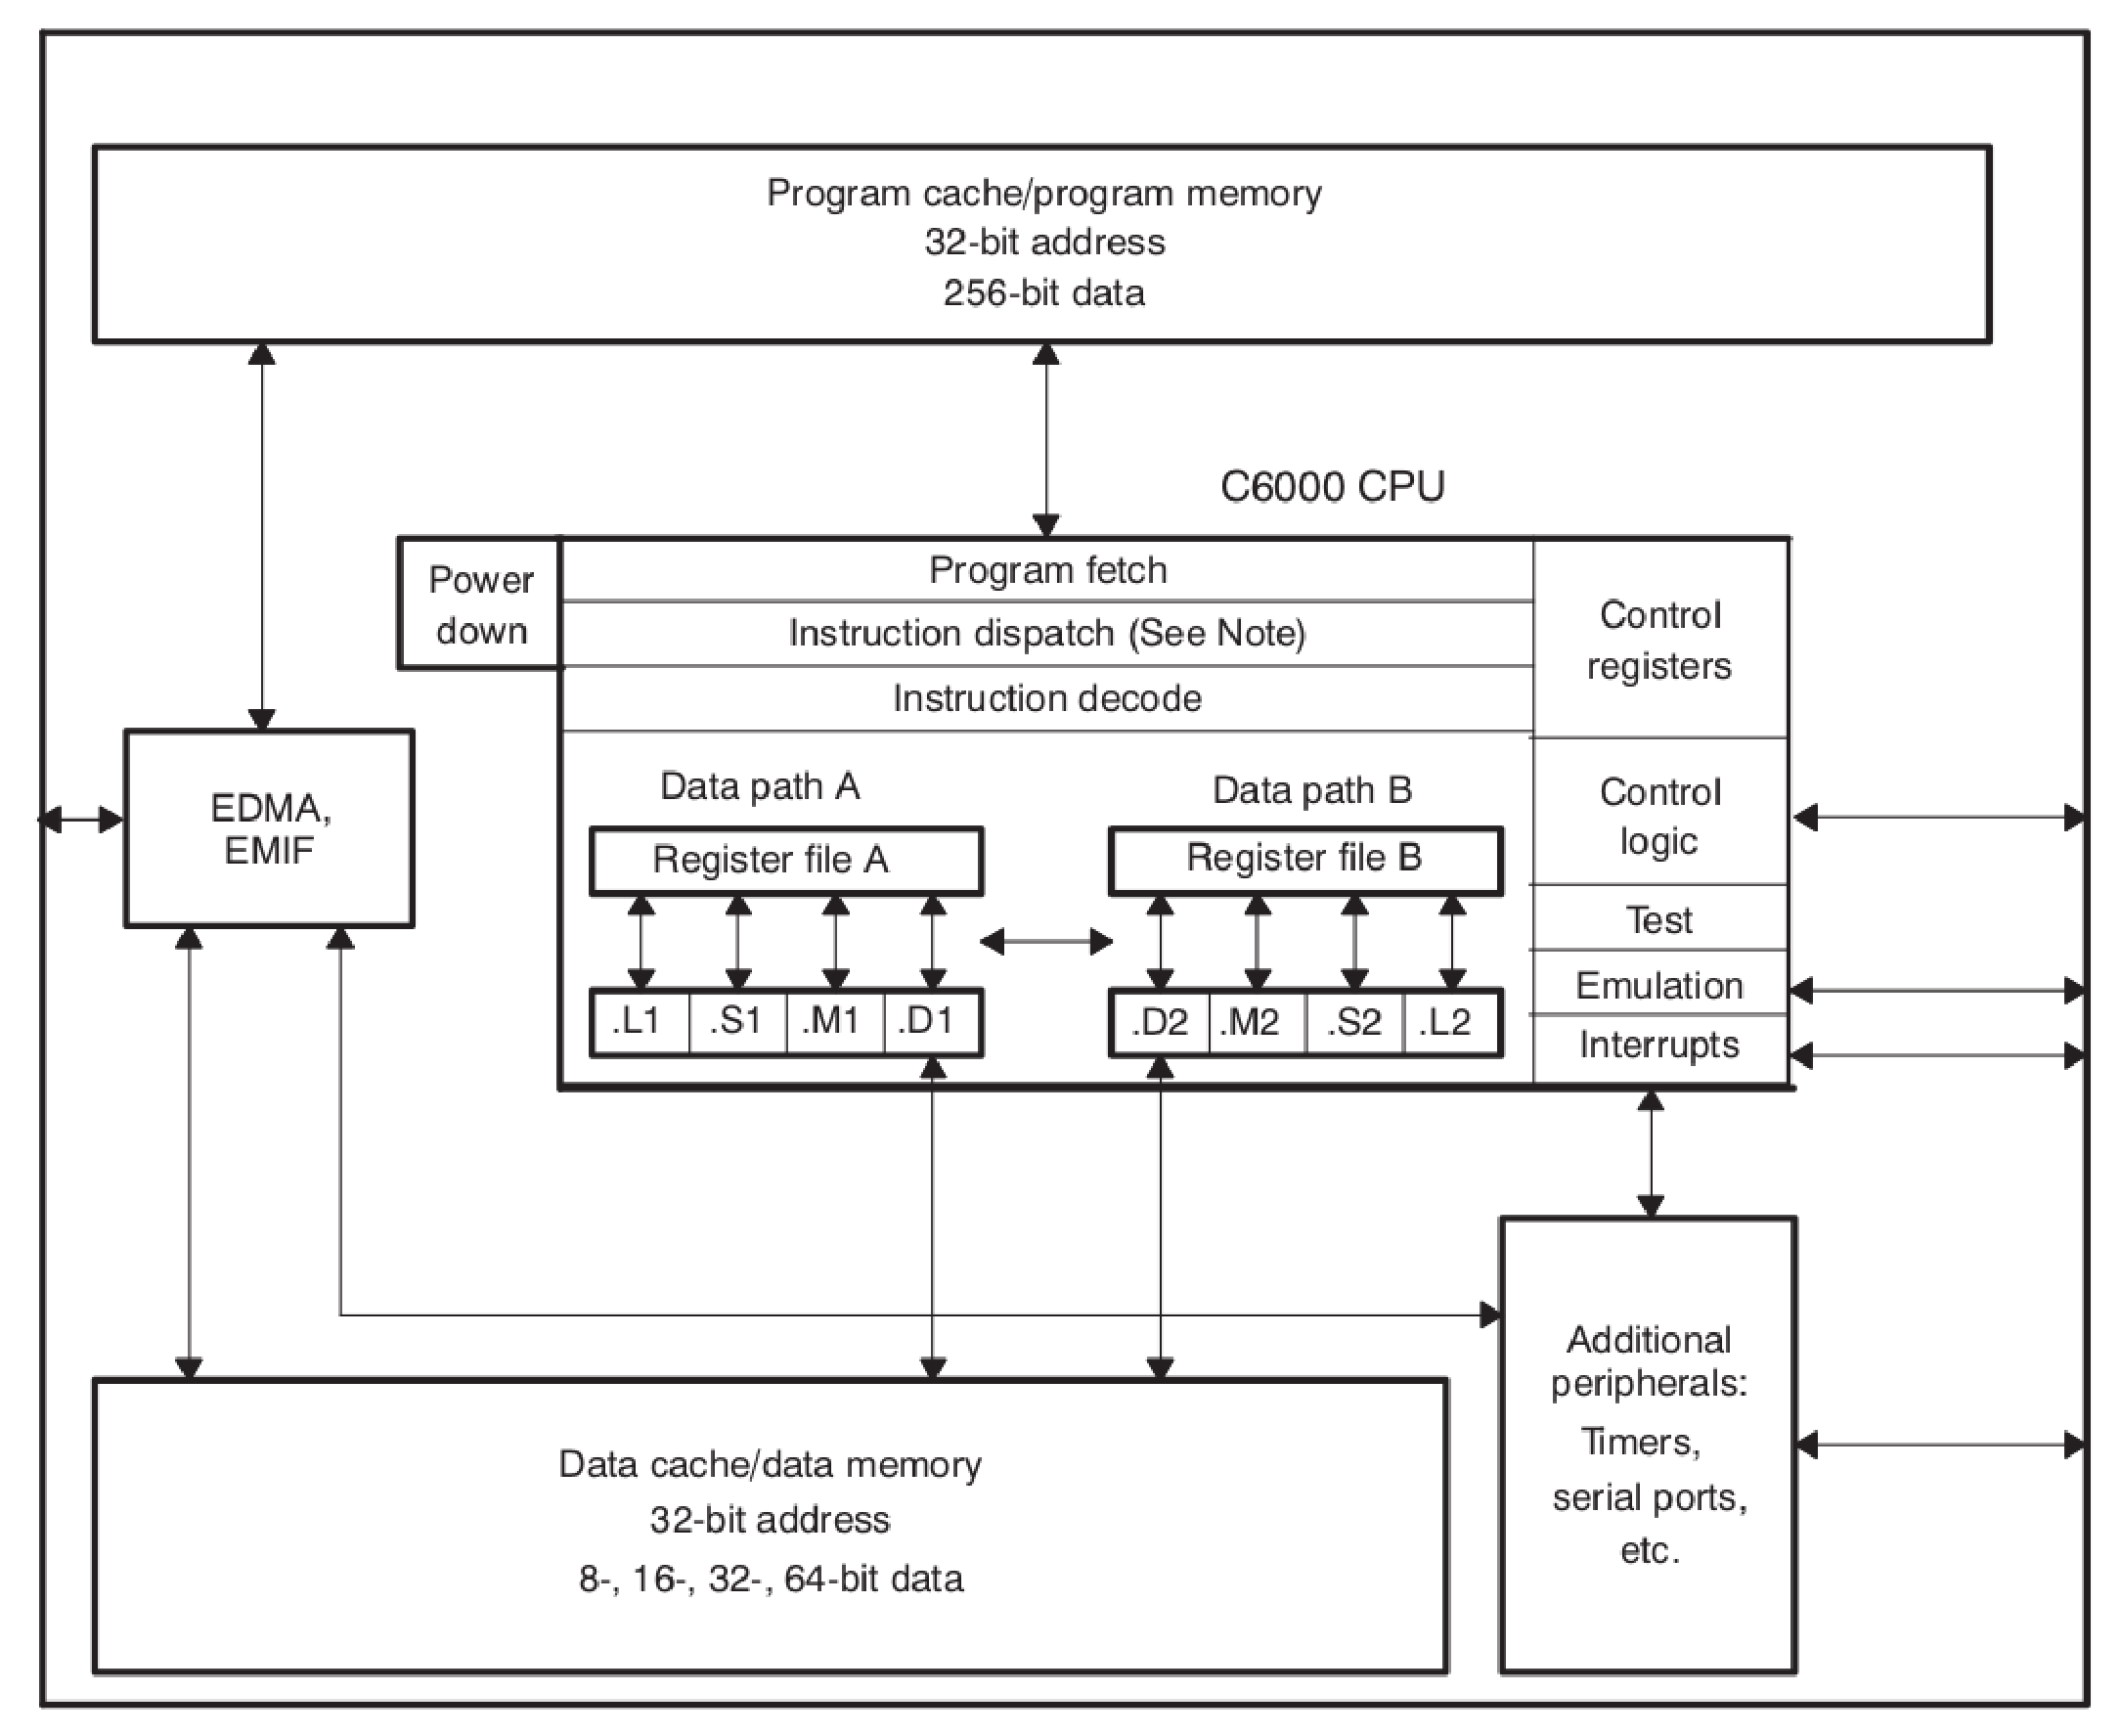
\includegraphics[scale=0.35]{mikroprozessoren2/TI-TMS320C64x.pdf}

Quelle: http://www.ti.com/lit/ug/spru732j/spru732j.pdf

\subsubsection{Vergleich Hardware- vs Software-Scheduling}
\begin{itemize}
	\item \textbf{Hardware-Scheduling}
	\begin{itemize}
		\item Bessere Speicherdisambiguierung, da zur Laufzeit die Adressen bekannt sind % TODO
		\item Sprungvorhersage, Precise Interrupts, kein Kompensierungscode
		\item Kompatibilität über mehrere Implementierungen
	\end{itemize}
	\item \textbf{Software-Scheduling}
	\begin{itemize}
		\item Größereres Befehlsfenster zum Finden von Parallelismus
		\item Geringerer Hardware-Aufwand
	\end{itemize}
\end{itemize}


\subsection{Explicitly Parallel Instruction Computing (EPIC)}
Gemeinsames Projekt von Hewlett-Packard und Intel (1994 angekündigt, ab 2001 auf dem Markt). Ziele:
\begin{itemize}
	\item 64 Bit Architektur: IA-64
	\item Explizite Spezifikation des Parallelismus im Maschinencode: \texttt{EPIC-Format} (entspricht dem VLIW-Prinzip)
	\item Bedingte Ausführung von Befehlen (Predication) sowie spekulative Ausführung von Ladeoperationen (Data Speculation)
	\item Großer Registersatz sowie skalierbarer Befehlssatz
	\item Sinnvolles Zusammenwirken zwischen Compiler und Hardware
	\item Reduzierung der Logikgatter, um den freigewordenen Platz besser zu nutzen (ermöglicht beispielsweise mehr ALUs, größere Caches, Reduzierung der Verlustleistung)
	\item Beispiele: Intel Itanium und Intel Itanium 2
\end{itemize}

\subsubsection{Intel IA-64}
\begin{itemize}
	\item \textbf{Registersatz}
	\begin{itemize}
		\item Integer Register: Sind als Stack organisiert (\texttt{GR32-GR127}) und unterstützen geschachtelte Prozessaufrufe. \texttt{GR0-GR31} sind immer zugreifbar und direkt adressierbar. \texttt{CFP} zeigt auf die Menge der Register, die für die aktuelle Prozedur verwendet werden
		\item Acht 64 Bit Branch-Register: Enthalten die Zieladressen für indirekte Verzweigungen
		\item 64 1 Bit Predicate-Register
	\end{itemize}
	\item \textbf{Befehlsformat (IA-64 ISA)}
	\begin{itemize}
		\item | Opcode (14 Bit) | Register 1 (7 Bit) | Register 2 (7 Bit) | Register 3 (7 Bit) | Predicate (6 Bit) |
		\item IA-64-Instruktionen werden vom Compiler in \textit{Bundles} gepackt (128 Bit Länge). \textit{Template} zeigt an, ob die Instruktionen parallel, eine Instruktion oder mehrere sequentiell oder benachbarte \textit{Bundles} parallel ausgeführt werden können. Beispiel Folie 112f \\ | Instruction 2 (41 Bit) | Instruction 1 (41 Bit) | Instruction 0 (41 Bit) | Template (5 Bit) |
	\end{itemize}
	\item \textbf{Befehlsgruppen}
	\begin{itemize}
		\item Instruktionen, die parallel ausführbar sind, werden vom Compiler in Gruppen zusammengefasst (\textit{instruction groups}). Innerhalb einer Gruppe können Befehle mit beliebigem Parallelitätsgrad und in beliebiger Reihenfolge ausgeführt werden
		\item \textit{Stops} markieren das Ende einer solchen Gruppe im Befehlsstrom
		\item Optimierungsziel: Verwenden von möglichst wenigen Gruppen mit einer möglichst hohen Anzahl an Befehlen innerhalb einer Gruppe
	\end{itemize}
	\item \textbf{Skalierbarkeit}
	\begin{itemize}
		\item Jedes \textit{Bundle} enthält drei Instruktionen für drei Funktionseinheiten
		\item Hat ein IA-64-Prozessor ein Vielfaches von jeweils drei Funktionseinheiten, dann können mehrere \texttt{Bundles} in ein Instruktionswort gepackt werden \(\rightarrow\) Skalierbarkeit bezüglich der Anzahl der Funktionseinheiten
	\end{itemize}
	\item \textbf{Predication: Bedingte Ausführung Befehlen ohne Verwendung von Sprungbefehlen}
	\begin{itemize}
		\item Evaluierung der bedingten Ausdrücke mit Hilfe von Compare-Operationen. Die Predicate-Register können mit Compare-Befehlen gesetzt werden. Jeder Befehl hat ein 6 Bit breites Predicate-Feld zur Angabe eines Predicate-Registers \(\rightarrow\) eleminiert Sprungbefehle
		\item Befehle werden nur ausgeführt, wenn das Predicate-Register \texttt{true} ist, anderenfalls wirken sie wie ein \texttt{NOP}
		\item Beispiel:\\ \texttt{cmp.eq p1, p2 = r1, r2;;\\(p1) sub r9 = r10, r11\\(p2) add r5 = r6. r7}
		\item Verfahren: Zur Laufzeit werden die voneinander unabhängigen Befehle angestoßen; der Prozessor führt die Befehle auf den möglichen Programmverzweigungen aus, speichert die Ergebnisse aber nicht endgültig; Überprüfen der Predicate Register und ggf. abschließen der Ausführung der Instruktionen (oder verwerfen des Ergebnisses)
		\item Implementierung
		\begin{itemize}
			\item Statische Vorschläge können in Verzweigungen kodiert werden und entscheiden, ob ein Eintrag von der dynamischen Branch Prediction Hardware alloziert wird
			\item Software und Hardware haben die gemeinsame Kontrolle über die Branch Prediction Hardware
		\end{itemize}
	\end{itemize}
	\item \textbf{Control Speculation}
	\begin{itemize}
		\item Ladebefehle werden vor Verzweigungen gezogen
		\item Problem (1): Verzweigungen schränken Code-Verschiebungen ein
		\item Lösung (1): Einführung von spekulativen Ladeoperationen VOR der Verzweigung mit \texttt{Speculation Check}, NACHDEM der Sprung ausgeführt worden ist. Alle Operationen, die spekulative Ergebnisse verwenden, können spekulativ ausgeführt werden (Beispiel Folie 118f)
		\item Problem (2): Ladeoperation kann nicht vor eine Speicheroption geschoben werden, da beide die selbe Adresse referenzieren könnten (Aliasing)
		\item Lösung (2): Vorgezogene Ladeoperation \texttt{ld.a} und Einfügen einer Load-Check-Operation \texttt{ld.c}. Bei \texttt{ld.a}-Operationen wird fortlaufend beobachtet, ob eine Speicheroperation die selbe Adresse referenziert, wie die \texttt{ld.a}-Operation. Falls keine Speicheroperation die Adresse von \texttt{ld.a} referenziert, ist \texttt{ld.c} eine Leeroperation, anderenfalls läd \texttt{ld.c} aus dem Speicher. Implementierung mit einer \texttt{Advanced Load Address Table}
	\end{itemize}
\end{itemize}

\subsubsection{Architektur Intel Itanium}
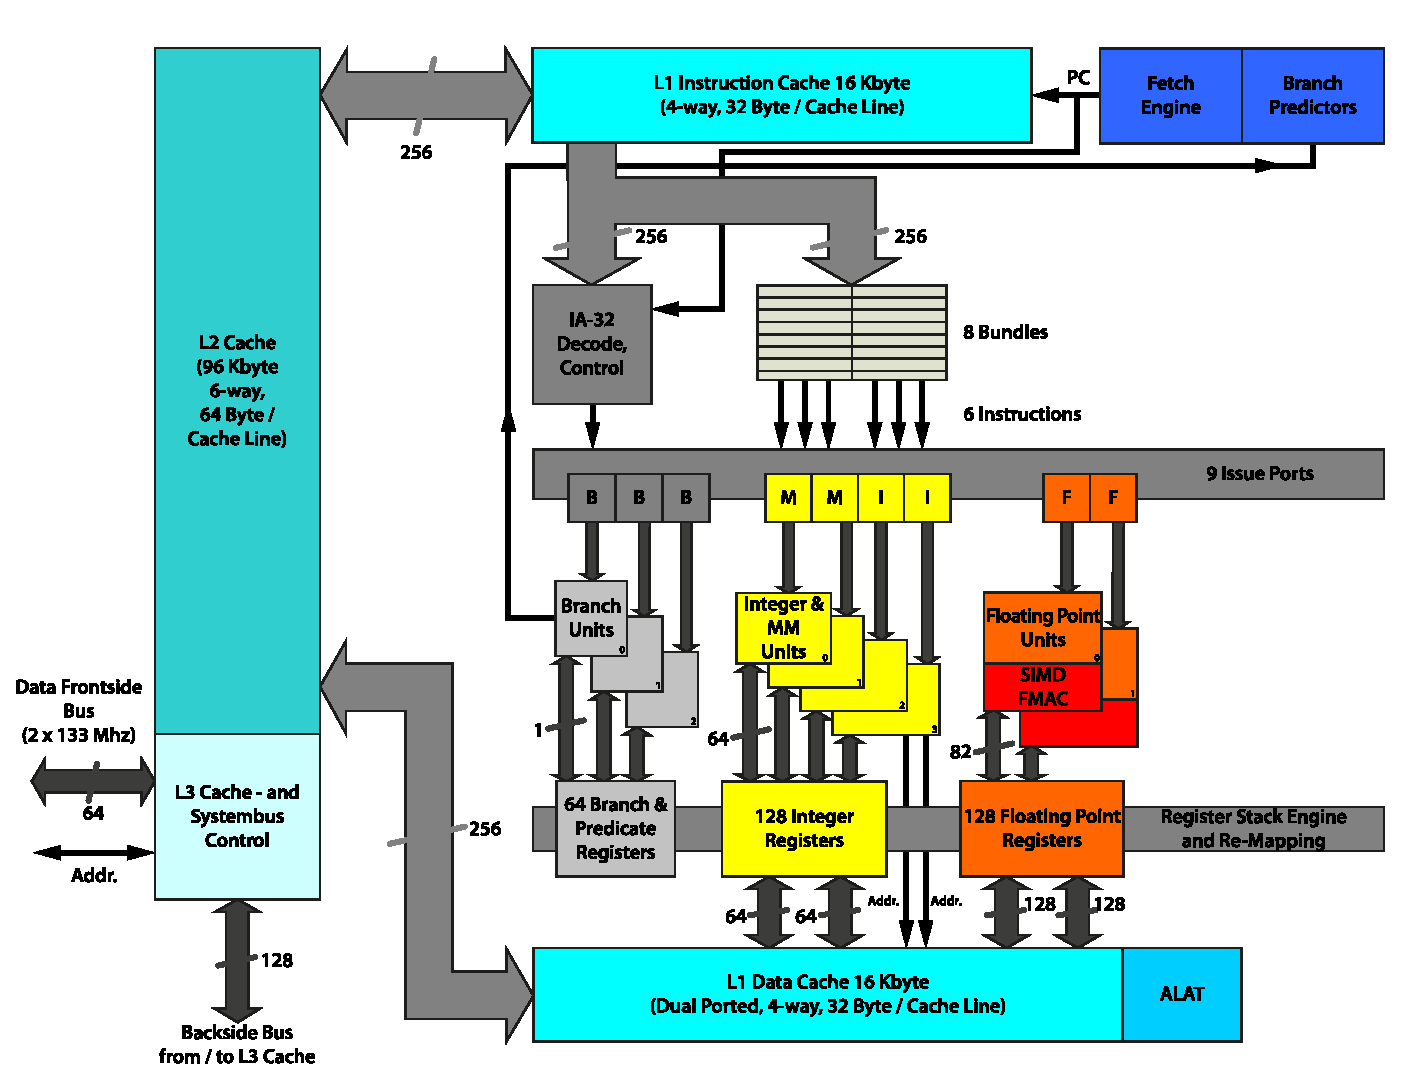
\includegraphics[scale=0.68]{mikroprozessoren2/Itanium_architecture.pdf}
% Quelle: https://upload.wikimedia.org/wikipedia/commons/a/ae/Itanium_architecture.svg



\section{Parallelismus auf Thread-Ebene: Multithreading}

\subsection{Einführung}

\subsubsection{Problem: Überbrücken von Wartezeiten}
\begin{itemize}
	\item \textbf{Wartezeiten durch}
	\begin{itemize}
		\item Konflikte aufgrund von echten Datenabhängigkeiten. Lösungen: Superskalartechnik, VLIW, EPIC
		\item Speicherzugriffe, die Cache-Fehler verursachen oder Zugriffe auf nicht-lokalen Speicher im Mehrprozessorsystem (zusätzlicher Aufwand zum Übertragen durch das Kommunikationsnetz)
		\item Ausführen von Befehlen mit langen Ausführungszeiten
		\item Anhalten des Prozessors zur Auflösung von Konflikten
		\item Synchronisation von parallelen Kontrollfäden
	\end{itemize}
	\item \textbf{Lösungsansatz}
	\begin{itemize}
		\item Idee: Füllen von Wartezyklen durch Umschalten auf andere Threads
		\item Allerdings: Hoher Aufwand bei Threadwechseln in "`konventionellen"' Prozessoren \(\rightarrow\) mehrfädige Prozessortechnik (Multithreading)
	\end{itemize}
\end{itemize}

\subsubsection{Mehrfädige Prozessortechnik (Multithreading)}
\begin{itemize}
	\item \textbf{Explizit mehrfädige Prozessoren}
	\begin{itemize}
		\item Überlappte Ausführung von Befehlen aus verschiedenen benutzerdefinierte Kontrollfäden (BS-Threads, Prozesse) in einer Pipeline \(\rightarrow\) bessere Auslastung der Pipeline
		\item Speicherung der Kontexte der verschiedenen Kontrollfäden: Mehrere getrennte Registersätze auf einem Chip sowie mehrere Befehlszähler in der Befehlsholeinheit
		\item Mehrere Kontexte von Befehlsfäden sind geladen: Umschalten der Ausführung zur Überbrückung von Ladezeiten. Erfolgt automatisch durch Hardware-unterstützte Wechselstrategie
		\item Multithreading in skalaren Prozessoren: Eine Befehlspipeline
		\item Multithreading in superskalaren Prozessoren: Mehrere Befehle von möglicherweise verschiedenen Befehlsströmen werden gleichzeitig zur Ausführung angestoßen. \textit{Simultanious Multithreading} (SMT) kombiniert Superskalartechnik mit Multithreading
		\item Anstoßen von Befehlen
		\begin{itemize}
			\item Anstoßen von Befehlen aus einem Kontrollfaden in einem Zyklus
			\begin{itemize}
				\item Interleaved Multithreading (cycle-by-cycle): In jedem Zyklus wird ein Befehl aus einem anderen Kontrollfaden geholt und ausgeführt
				\item Blocked Multithreading: Die Befehle eines Threads werden solange ausgeführt bis ein Ereignis eintritt, das eine lange Wartezeit nach sich zieht
			\end{itemize}
			\item Anstoßen von Befehlen aus mehreren Kontrollfäden in einem Zyklus: Befehle aus mehreren Kontrollfäden werden gleichzeitig zur Ausfürhung auf einem superskalaren Prozessor angestoßen (\textit{Simultaneous Multithreading})
		\end{itemize}
		\item Embedded Systems: Prozessor bietet Algorithmen zur Steuerung der einzelnen Programmthreads. Sie können durch entsprechende Befehle in einen Wartezustand versetzt und durch Hardware-Ereignisse aufgeweckt werden. Hierdurch sind sehr schnelle Reaktionen des Systems möglich, da im Gegensatz zum klassischen Hardware-Interrupt keinerlei Overhead beim Kontextwechsel notwendig ist und ohne die Leistung des Systems merklich zu beeinflussen.\footnote{\url{https://de.wikipedia.org/wiki/Hardwareseitiges_Multithreading\#Multithreadingf.C3.A4hige_Prozessoren_f.C3.BCr_eingebettete_Anwendungen}}
	\end{itemize}
	\item \textbf{Implizit mehrfädige Prozessoren} % TODO
	\begin{itemize}
		\item Erzeugen dynamisch Kontrollfäden aus einem Programm (single-threaded)
		\item Thread-level Spekulation: Führt die Kontrollfäden spekulativ parallel aus und verwirft ggf. spekulativ berechnete Ergebnisse
	\end{itemize}
\end{itemize}
% Vgl der Prozessortechniken: Folie 137-139


\subsection{Multithreading-Techniken}

\subsubsection{Interleaved Multithreading (IMT, cycle-by-cycle, fine-grain Multithreading)}
\begin{itemize}
	\item Idee: Verhinderung von Pipelinekonflikten
	\item Der Prozessor wählt aus einer Anzahl geladener Kontrollfäden einen ausführbereiten aus und gibt einen Befehl in die Pipeline. Schema: \texttt{[1,2,3,4,1,2,3,4,...]}
	\item Es wird immer erst ein neuer Befehl eines Threads in die Pipeline getan, wenn der vorherige komplett abgearbeitet worden ist (gilt auch bei Speicherzugriff) \(\rightarrow\) Elimination von Pipelinekonflikten
	\item Aufwand zum Thread-Wechseln beträgt null Zyklen
	\item Idealerweise gibt genau so viele Threads wie Taktzyklen für Speicherzugriffe benötigt werden. Anderenfalls werden Wartezyklen eingebaut
	\item Reduziert die Ausführungszeit eines Kontrollfadens zugunsten des Durchsatzes vieler Threads
	\item \textbf{Dependence look-ahead Technik}
	\begin{itemize}
		\item Begrenzte Anzahl Befehlen desselben Kontrollfadens kann überlappend ausgeführt werden
		\item Compiler kennzeichnet im Opcode eines Befehls die Anzahl der von diesem Befehl unabhängigen Folgebefehle \(\rightarrow\) unabhängige Befehle können zum Auffüllen benutzt werden
		\item Bessere Auslastung der Ressourcen, falls nicht genügend Kontrollfäden zur Verfügung stehen
	\end{itemize}
\end{itemize}

\subsubsection{Blocked Multithreading (BMT, coarse-grain Multithreading)}
\begin{itemize}
	\item Befehle eines Kontrollfadens werden solange ausgeführt, bis eine höhere Leistung bei der Ausführung oder höherer Aufwand beim Thread-Wechseln (Flush der Pipeline) notwendig ist
	\item \textbf{Statische Modelle zum Threadwechseln}
	\begin{itemize}
		\item Explicit switch
		\begin{itemize}
			\item Ein Thread-Wechsel tritt jedes Mal auf, wenn ein bestimmter Befehl im Befehlsstrom auftritt
			\item Thread-Wechsel werden durch den Compiler kodiert und kann bereits in der Befehlsbereitstellung erkannt und durchgeführt werden \(\rightarrow\) verringerter Aufwand für den Kontextwechsel
		\end{itemize}
		\item Implicit switch
		\begin{itemize}
			\item Jeder Befehl wird einer Befehlsklasse zugeordnet. Diese bestimmt, ob ein Kontextwechsel notwendig ist
			\item Beispiele für Befehlsklassen, die Kontextwechsel auslösen: Lade-, Speicher- und Sprungbefehle
			\item Techniken
			\begin{itemize}
				\item Switch-on-load: Kontextwechsel nach jedem Ladebefehl. Bei vorhandenem Datencache erfolgt der Kontextwechsel öfters als notwendig
				\item Switch-on-store: Kontextwechsel nach jedem Schreibbefehl. Bietet sich nur an, wenn sequentielle Speicherkonsistenz implementiert werden soll, da anderenfalls ein Schreibpuffer vorhanden ist
				\item Switch-on-branch: Kontextwechsel nach jeder Verzweigung. Damit kann auf Speungvorhersage und spekulative Ausführung verzichtet werden, ist in modernen Prozessoren allerdings eher ungewöhnlich
			\end{itemize}
		\end{itemize}
	\end{itemize}
	\item \textbf{Dynamische Modelle zum Threadwechseln}
	\begin{itemize}
		\item Kontextwechsel wird durch ein dynamisch auftretendes Ereignis ausgelöst. Alle Instruktionen in der Pipeline bis zu der Phase, die den Kontextwechsel ausgelöst hat werden verworfen \(\rightarrow\) höherer Aufwand für den Kontextwechsel
		\item \textbf{Modelle}
		\begin{itemize}
			\item Switch-on-cache-miss: Wird erst spät erkannt, deswegen müssen alle nachfolgenden Befehle in der Pipeline verworfen werden
			\item Switch-on-signal: Kontextwechsel beim Auftreten eines speziellen Signals, beispielsweise Interrupts, Trap, etc.
			\item Switch-on-use: Kontextwechsel, falls ein Befehl einen Wert verwenden will, der (nach einer Ladeoperation) noch nicht bereit gestellt ist. Für die Implementierung wird ein Valid-Bit hinzgefügt das anzeigt, ob ein Wert nach einer Ladeoperation bereits bereitsteht
			\item Conditional-switch: Bindet expliziten Switch-Befehl an eine Bedingung (ersetzt damit switch-on-use). Ein Kontextwechsel erfolgt nur dann, wenn diese Bedingung erfüllt ist. Beispielsweise bei Lade- und Speicherbefehlen erfolgt der Kontextwechsel bei einem Cache-Miss
		\end{itemize}
	\end{itemize}
\end{itemize}

\subsubsection{Simultaneous Multithreading (SMT)}
\begin{itemize}
	\item \textbf{Kombiniert Superskalartechnik mit Multithreading}
	\begin{itemize}
		\item Verwendet Hardware-Ressourcen für das gleichzeitige Festhalten mehrerer Kontexte, die alle gleichzeitig aktiv sind
		\item In jedem Zyklus können mehrere Befehle aus verschiedenen Kontrollfäden gleichzeitig angestoßen werden
		\item Thread level Parallelismus: Multithreaded parallele Programme. Mehrere unabhängige Programme in einer Multiprogramming-Umgebung
		\item Mehrere Registersätze auf einem Prozessor
		\item Wartezyklen, die von einer Instruktion aus einem Kontrollfaden verursacht werden, können durch das Ausführen von Befehlen aus anderen Kontrollfäden verdeckt werden
	\end{itemize}
	\item \textbf{Organisation der Hardware}
	\begin{itemize}
		\item Gemeinsame Hardware-Ressourcen (resource sharing): Die Befehle aus den verschiedenen Kontrollfäden können auf alle Ressourcen gemeinsam zugeifen. Beispielsweise Befehlsholpuffer, RATs, Befehsfenster, Retire, etc.
		\item Minimaler zusätzlicher Hardwareaufwand für superskalaren Prozessor: Zusätzlich Thread-Tag für jede interne Befehlsdarstellung, mehrere Registersätze, Befehlsholen und -abschließen (retire) für mehrere Kontrollfäden
		\item Replikation von Ressourcen
		\begin{itemize}
			\item Replizieren der internen Puffer von superskalaren Prozessoren. Jeder Kontrollfaden ist einem Puffer zugeordnet
			\item Die Einheiten zum Befehlholen, -dekodieren und -abschließen
			\item Befehle können aus verschiedenen Befehlsfenstern gleichzeitig zur Ausführung angestoßen werden
		\end{itemize}
	\end{itemize}
\end{itemize}
% Siehe Diagramm auf Folie 153


\subsection{Fallstudien}

\subsubsection{Fallstudie: Intel Hyperthreading Technology}
\begin{itemize}
	\item Simultanious Multithreading für Intel-Xeon Prozessoren
	\item Eingeführt 2004 mit dem Intel Pentium 4
	\item Ein physikalischer Prozessor erscheint wie zwei logische Prozessoren. Die physikalischen Ausfürhungsressourcen werden zwischen den logischen Prozessoren geteilt \(\rightarrow\) aus Softwaresicht können Prozesse und Threads auf zwei Prozessoren aufgeteilt werden
	\item Unterschiede zum "`klassischen"' SMT-Modell: Gemeinsame Funktionseinheiten und Caches sowie statische Aufteilung von Queues und Puffer, einschließlich der Instruction Schedule Queue
\end{itemize}

\subsubsection{Fallstudie: Sun UltraSPARC T1, T2 (Niagara)}
\begin{itemize}
	\item \textbf{Niagara 1}
	\begin{itemize}
		\item Cycle-by-cycle Multithreading: LRU-Strategie für die Auswahl der bereiten Threads. Falls vier Threads bereit sind: Round-Robin-Strategie in jedem Taktzyklus. Falls ein Thread warten muss, wird er aus der RR-Strategie herausgenommen, bis er wieder bereit ist
		\item Leistungsvergleich Single threaded vs. Four threaded: 21 \% Effiziens gegenüber 72 \%
	\end{itemize}
	\item \textbf{Niagara 2}
	\begin{itemize}
		\item Einführung einer zweiten Pipeline (dual execution pipeline). Beide Pipelines unterstützen vier Kontrollfäden
	\end{itemize}
\end{itemize}

\subsubsection{Pipeline Niagara 1}
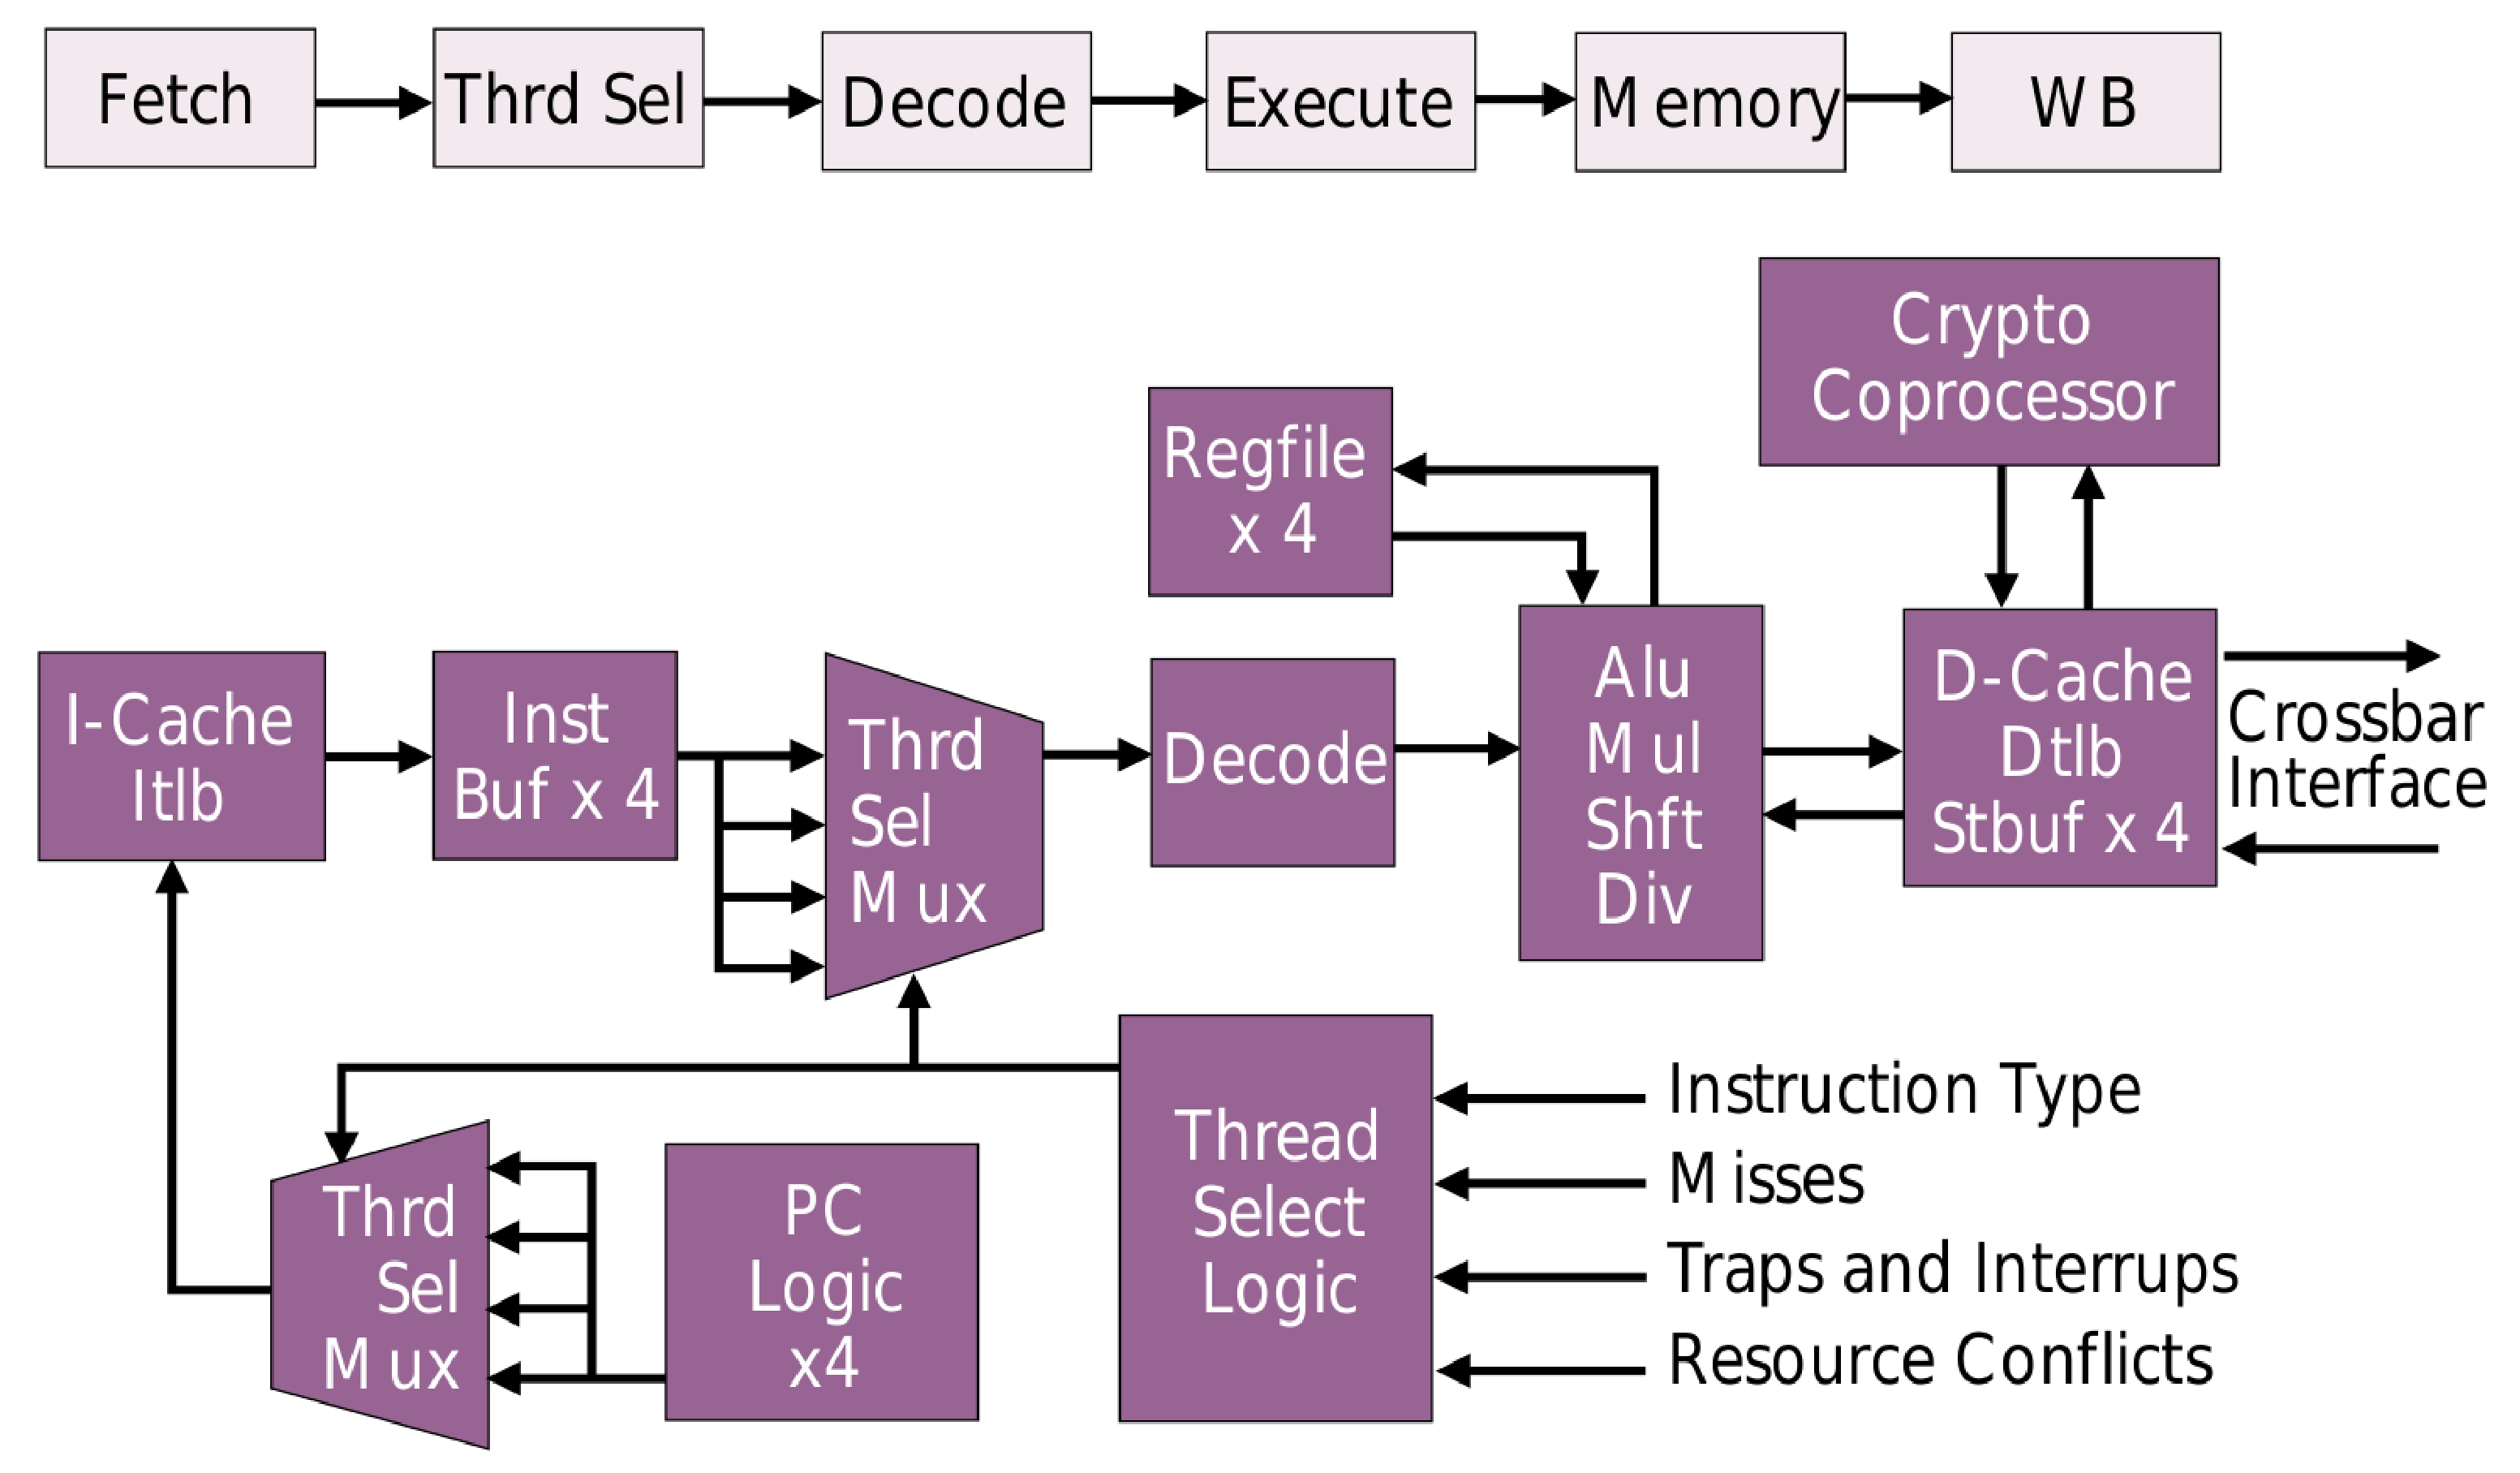
\includegraphics[scale=0.3]{mikroprozessoren2/Niagara1.pdf}

Niagara 1 core pipeline. This unit handles basic integer ALU operations plus shifts and integer multiply and divide. The only features that distinguish it from a basic 1980s scalar RISC pipeline are the thread-select stage and the cryptographic coprocessor. The cryptographic coprocessor shares the crossbar interface with the L1 D-cache but does not modify its contents, streaming data directly out of and back into the L2 cache.\footnote{\url{Quelle: Niagara 2 Opens the floodgates (11/06/6-01)}}

\subsubsection{Leistungsvergleich Single threaded vs. Four threaded}
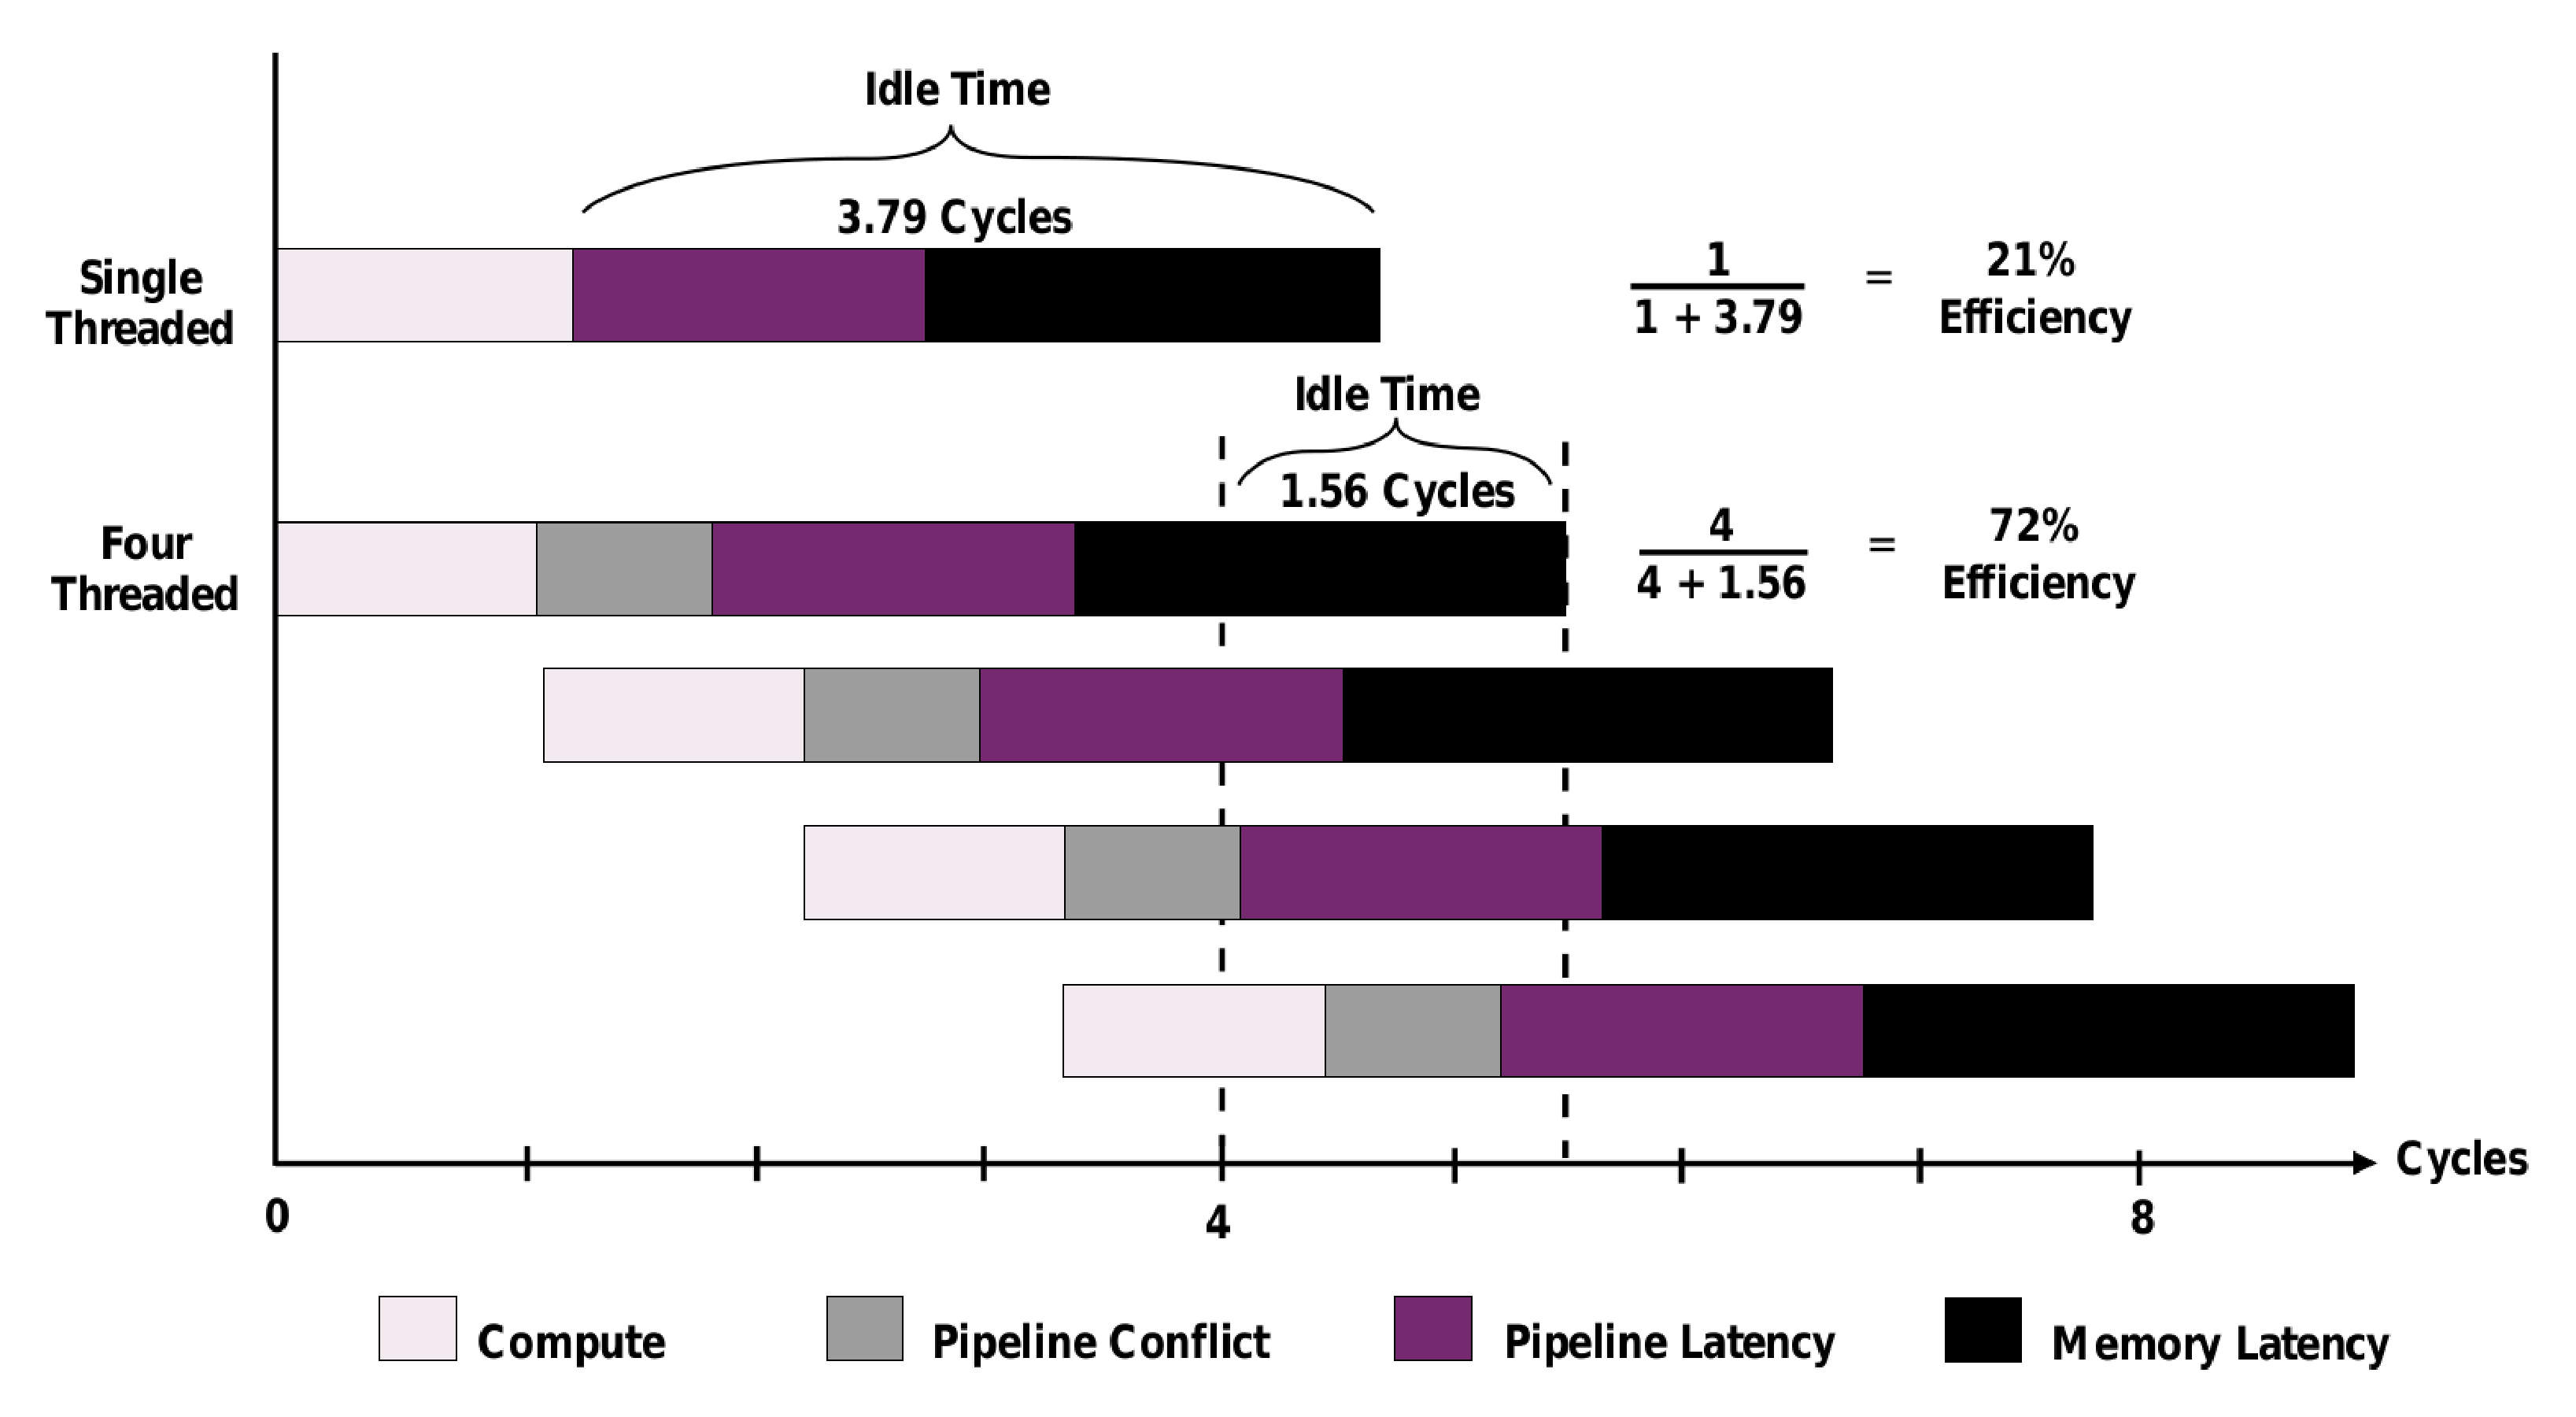
\includegraphics[scale=0.25]{mikroprozessoren2/Niagara1_Leistungsvergleich.pdf}

Here is a measured example of Niagara 1’s execution efficiency, drawn from an analysis of the SPECjbb benchmark program that Sun provided at the 2006 International Solid-State Circuits Conference (ISSCC). Although the four-way multithreaded Niagara 1 core is not perfectly efficient, it is far more efficient than any single-threaded core. The idleness of nearly 80 \% shown for a single-threaded core on this benchmark is shocking in its own right, but it is only the tip of the iceberg of inefficiency where superscalar designs are concerned. For a superscalar processor, most busy cycles leave some execution slots unfilled, while every idle cycle leaves all its multiple execution slots unfilled. Source: A. S. Leon et al., "`A Power-Efficient High Throughput 32-Thread SPARC Processor,"' ISSCC06, Paper 5.1\footnote{\url{Quelle: Niagara 2 Opens the floodgates (11/06/6-01)}}

\subsubsection{Erweiterungen beim Niagara 2}
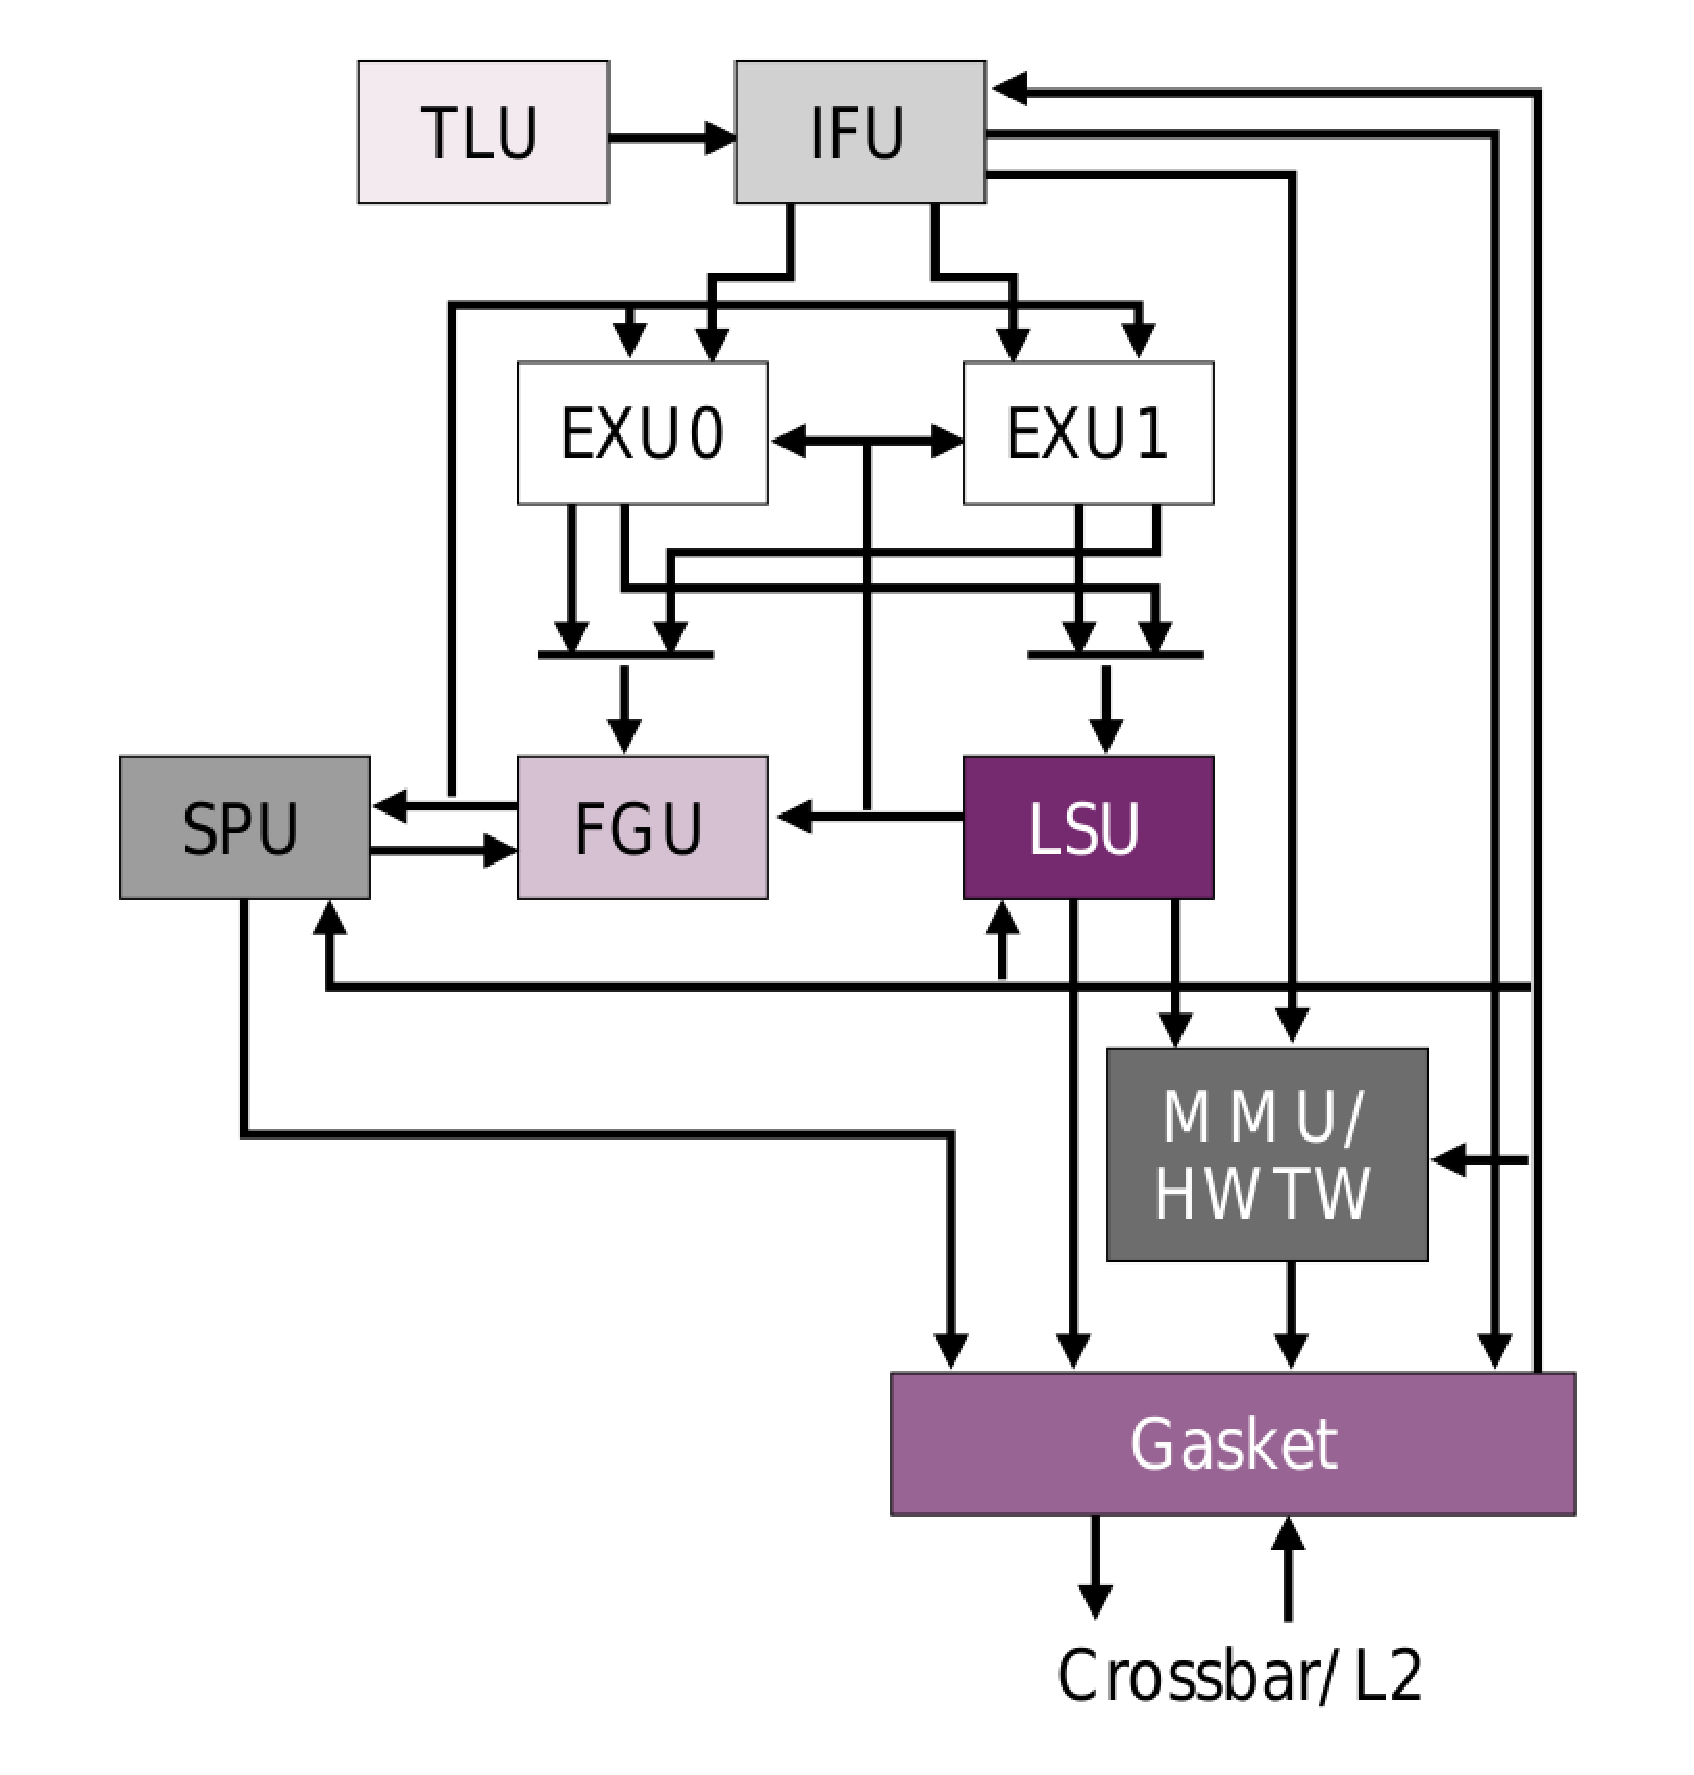
\includegraphics[scale=0.35]{mikroprozessoren2/Niagara2_Erweiterungen.pdf}

In Niagara 2 cores, the most visible changes are the dual execution pipelines (EXU0 and EXU1), each supporting four threads, and the new FGU. Other units were present in the Niagara 1 core. TLU is the trap logic unit (for interrupt and trap handling); IFU is the instruction-fetch unit (which includes the 16KB I-cache); SPU is the stream processing or crypto unit (which now shares resources with the FGU); and LSU is the load/store unit (which includes the 8KB D-cache). The memory management unit (MMU) includes hardware table walk (HWTW) for page sizes ranging from 8KB to 256MB. The gasket is the interface to the crossbar, which handles all traffic in and out of the core.\footnote{\url{Quelle: Niagara 2 Opens the floodgates (11/06/6-01)}}



\section{Multicore/Manycore}

\subsection{Multicore, Manycore}

\subsubsection{Merkmale von Multicore-Architekturen}
\begin{itemize}
	\item Gemeinsamer oder privater Speicher
	\item \textbf{Verbindungsstrukturen}
	\begin{itemize}
		\item Cache-kohärenter Chip-Multiprozessor: Transportiert Nachricht des Cache-Kohärenzprotokolls und Cache-Zeilen zwischen Prozessorkernen (On-Chip-Netzwerk)
		\item Merkmale
		\begin{itemize}
			\item Topologie (Wie werden die Knoten verbunden): Beispielsweise Bus-System (IBM Power5 oder AMD Opteron), Ringnetzwerk (IBM Cell Broadband Engine) oder Gitternetz (MIT Raw Processor)
			\item Routing beim MIT Raw Processor: Mesh-Netzwerk, bei dem jeweils die benachbarten Kerne direkt miteinander kommunizieren
		\end{itemize}
	\end{itemize}
\end{itemize}

\subsection{Prallele Architekturen}
\begin{itemize}
	\item \textbf{Programmiermodell}
	\begin{itemize}
		\item Abstraktion einer virtuellen Maschine, auf welcher der Anwender sein Programm formuliert
		\item Spezifiziert, wie Teile des Programms parallel abgearbeitet werden, wie Informationen ausgetauscht werden und welche Synchronisationsoperationen verfügbar sind, um die Aktivität zu koordinieren
		\item Anwendungen werden auf der Grundlage eines parallelen Programmiermodells formuliert
	\end{itemize}
	\item \textbf{Datenparallelismus}
	\begin{itemize}
		\item Gleichzeitiges Ausführen von Operationen auf getrennten Elementen einer Datenmenge (Feld, Matrix)
		\item Typischerweise in Vektorprozessoren, heute auch vielfach in Mikroprozessoren (Intel MMX oder SSE, AMD 3Dnow!, IMB VMX im PowerPC, Sparc VIS). Spezielle Form: Single-Instruction-Multiple-Data
	\end{itemize}
	\item \textbf{Funktionsparallelismus/Task-level parallelism}
	\begin{itemize}
		\item Unabhängige Funktionen werden auf verschiedenen Prozessoren ausgeführt
		\item Beispiel Video-Streaming: Verschiedene Formen werden auf einen Strom von Daten angewendet
		\item Funktionen können Funktions-Pipeline bilden
	\end{itemize}
	\item \textbf{Gemeinsamer Speicher (Shared Memory)}
	\begin{itemize}
		\item Gemeinsame genutzer Speicherbereich
		\item Kommunikation und Koordination von Prozessen über gemeinsame Variablen
		\item Kommunikationsarchitektur: Verwendung konventioneller Speicheroperationen für die Kommunikation gemeinsamer Adressen. Die Synchronisationsoperationen sind atomar
	\end{itemize}
	\item \textbf{Multiprozessor mit gemeinsamem Speicher}
	\begin{itemize}
		\item Uniform Memory Access: Speicherarchitektur in Multiprozessorsystemen, bei denen es nur einen globalen Speicher gibt, auf den alle Prozessoren einheitlich zugreifen
		\item Zugriff erfolgt über ein Verbindungsnetzwerk
	\end{itemize}
	\item \textbf{Chip Multiprocessors (Eigenschaften)}
	\begin{itemize}
		\item Gemeinsamer L2-Cache über gemeinsamen Bus
		\item Kohärenz (verhindert, dass die einzelnen Caches für dieselbe Speicheradresse unterschiedliche (inkonsistente) Daten zurückliefern\footnote{\url{https://de.wikipedia.org/wiki/Cache-Koh\%C3\%A4renz}}) für L1-Caches wird durch Bus-Snooping hergestellt (stetige Kontrolle der Speicher-Adressleitungen (Bus), um eventuellen Konflikten zwischen Speicher- und Cacheinhalten vorzubeugen\footnote{\url{https://de.wikipedia.org/wiki/Bus_snooping}})
		\item Beispiel: Pentium IV Dual Core Prozessor
	\end{itemize}
\end{itemize}

\subsubsection{Chip Multiprocessors: Ringbasierte CMPs}
\begin{itemize}
	\item Knoten (Prozessorkerne und L2-Bank) sind über einen Ring verbunden
	\item Mehrere Abfragen können auf verschiedenen Links überlappend bearbeitet werden
	\item Router in jedem Knoten leiten die Pakete weiter
	\item Geschwindkeitsvorteil gegenüber Bussen: Ringe können schneller getaktet werden
	\item Snooping-Protokolle: Kohärenzanfragen besuchen einen jeden Knoten. Anforderungen werden an alle Knoten verschickt. Owner antworten mit dem Block bei einem Fehlzugriff (Kohärenztransaktionen benötigen einen Umlauf)
	\item Beispiel: Intel Core i7
\end{itemize}


\subsection{Parallele Programmiermodelle: OpenMP}

\subsubsection{Einführung}
\begin{itemize}
	\item Schnittstelle für die Shared-Memory-Programmierung in C, C++ und Fortran auf Multiprozessorsystemen
	\item Parallelisiert Programme auf der Ebene von Schleifen, die in verschiedenen Threads ausgeführt werden und unterscheidet sich dadurch von anderen Ansätzen (z. B. MPI), bei denen ganze Prozesse parallel laufen und durch Nachrichtenaustausch zusammenwirken\footnote{\url{https://de.wikipedia.org/wiki/OpenMP}}
	\item Fork/Join-Ausführungsmodell: Betritt ein Thread eine parallele Region dann wird er Master-Thread und erzeugt ein Thread-Tem. Ersterer  übernimmt die Kontrolle und startet die parallele Abarbeitung durch Thread-Team (Fork) mit abschließender Barrieren-Synchronisation (Join). Danach Weiterfürhung durch den Master-Thread
	\item \textbf{Parallele Regionen}
	\begin{itemize}
		\item Fork-Join-Modell (s.o.)
		\item Threadzahl: Vorgabe durch Umgebungsvariable oder durch explizites Setzen oder durch Dynamisierung druch OpenMP
		\item Verschachtelung: Erzeugen neuer Teams
	\end{itemize}
	\item \textbf{Parallelisierungsderektiven}
	\begin{lstlisting}[frame=single,numbers=left,mathescape,language=C]
foo(int a[]) {
  #pragma omp for
  for (int i=1; i<n; i++)
    a[i]=i
}

main() {
  int a[100]

  #pragma omp parallel
  {
    foo(a)
  }
}
	\end{lstlisting}
	\begin{itemize}
		\item Parameter zur Steuerung: Definition privater oder gemeinschaftlicher Variablen, Werteübernahme in/aus paralle(r) Region, Zusammenführung von Werten. Standardverhalten bei lokalen Variablen: Privat.
	\end{itemize}
	\item \textbf{Gemeinsame und private Daten}
	\begin{itemize}
		\item Gemeinsame Daten: In allen Threads sichtbar, Referenzen beziehen sich auf identische Adressen
		\item Private Daten: Nur innerhalb eines Threads sichtbar. Keine Wechselwirkung mit anderen Threads
	\end{itemize}
	\item \textbf{Datenkonstrukte}
	\begin{itemize}
		\item \texttt{\#pragma omp threadprivate (list)}
		\item Aufsetzen von Thread-internen Variablen
		\item Jeder Thread erhält dabei eine lokale Kopie. Schreibvorgänge anderer Threads sind unsichtbar
		\item Übernahme aus dem Master-Thread möglich, sonst undefiniert
		\item Unterschied zu \texttt{PRIVATE}: Bisher Deklaration in jeder Routine mit blockspezifischem oder globalen Scope. Bei \texttt{PRIVATE} erfolgt eine einmalige Definition zu Beginn einer Region
	\end{itemize}
	\item \textbf{Work-Sharing-Konstrukte}
	\begin{itemize}
		\item Aufteilung der Ausführung des eingeschlossenen Code-Regionen innerhalb des Thread-Teams
		\item Do/for: Sharing der Schleifeniterationen
		\item Sektion: Zerlegung in separate Sektionen. Ausführung einer Sektion pro Thread
	\end{itemize}
	\item Parallele Schleifen: \texttt{for}-Direktive
	\begin{itemize}
		\item Verteilung der Iterationen an alle Threads
		\item Scheduling gemäßg gewählter Strategie
		\item Implizite Barriere zur Synchronisation sowie Definition von Reduktionsoperatoren für Variablen zur Zusammenführung
	\end{itemize}
	\item Ablaufsteuerung % TODO: Finde Beispiele
	\begin{itemize}
		\item Geordnetes Konstrukt (\texttt{\#pragma omp [for] ordered}): Ausführung in Reihenfolge wie bei sequentieller Abarbeitung. Kein "`Überholen"' innerhalb der parallelen Region
		\item Sektionen \texttt{\#pragma omp section[s] ordered}): Kapseln von Threads (jede Sektion wird von einem Thread ausgeführt). Synchronisation durch implizite Barriere
		\item Kritische Sektionen \texttt{\#pragma omp critical [name]}): Kritische Sektionen können nur von einem Thread ausgeführt werden. Es wird gewartet bis die kritische Sektion frei ist, dann erfolgt die weitere Abarbeitung. Synchronisation durch implizite Barriere
	\end{itemize}
	\item \textbf{Synchronisationskonstrukte} % TODO: Beispiele
	\begin{itemize}
		\item \texttt{MASTER}: Ausführung durch einen einzelnen Thread. Implizite Synchronisation aller Threads am Ender der Master-Region
		\item \texttt{SINGLE}: Ausführung durch einen einzelnen Threads mit Parameter zur Variablenverwaltung
		\item \texttt{BARRIER}: Synchronisation aller Threads eines Teams. Es wird gewartet bis alle Threads die Barriere erreicht haben
		\item \texttt{ATOMIC}: Ausführen einer atomaren Speicheroperation. Beispiele: Variablenänderung oder Vergleichsoperationen
		\item \texttt{FLUSH}: Synchronisationspunkt zum Erzwingen einer konsistenten Speichersicht. Erfolgt explizit bei Barrieren, beim Betreten und Verlassen kritischer Sektionen und beim Verlassen bestimmter Blöcke (\texttt{PARALLEL, FOR, SECTIONS, SINGLE})
	\end{itemize}
	\item Laufzeitumgebung: Verschiedene Funktionen zum Auslesen/Setzen von Threadzahlen oder Teamgrößen oder zum Ermitteln der Prozessoranzahl oder der Threadanzahl
\end{itemize}


\subsubsection{Parallele Architekturen: No Remote Memory Access (NoRMA)}
\begin{itemize}
	\item Jede CPU verfügt über einen eigenen Cache, eigenen Speicher sowie ein separates Interface zum Interconnection Network. Der Speicher ist statisch partitioniert, es gibt keinen globalen Speicherbereich. Austausch von Informationen zwischen den CPUs per Message-Passing
	\item NoC: Gitterstruktur
	\item Zugriffe auf entfernte Speichermodule nur per Message-Passing möglich
	\item Vorteil: Extrem große Konfigurationen möglich
	\item \textbf{Kommunikationsarchitektur}
	\begin{itemize}
		\item Verwendung von korrespondierenden Send- und Receive-Operationen
		\item Send: Spezifiziert einern lokalen Datenpuffer und einen Empfangsprozess auf einem entfernten Prozessor
		\item Receive: Spezifiziert einen Sendeprozess auf einen lokalen Datenpuffer, in dem die Daten ankommen
	\end{itemize}
	\item Definition von Parallelisierungsprozessen mit Hilfe von \texttt{CREATE, SEND, RECEIVE} und \texttt{BARRIER}
\end{itemize}


\section{Heterogene Parallelsysteme}

\subsection{Einführung}
\begin{itemize}
	\item \textbf{Definition}
	\begin{itemize}
		\item Verbund von Instanzen mit unterschiedlichen Eigenschaften
		\item Vorteilhaft, wenn eine Klasse nicht für alle Anforderungen optimal geeignet ist
		\item Einsatz mit unterschiedlichen Zielen. Beispielsweise um die Leistung, Energieeffiziens oder Robustheit zu erhöhen
		\item Heterogene Netzwerke: Knoten mit unterschiedlicher Hardware oder Betriebssystem. Beispielsweise neue Aufbaustufe eines Clusters mit besseren Prozessoren
		\item Heterogenität innerhalb eines Knotens: Beispielsweise unterschiedliche CPUs oder Beschleuniger, die per QuickPath, Hypertransport oder PCIe verbunden sind. Meist CPUs in Kombination mit dedizierten Grafikkarten odr FPGAs
		\item Heterogenität auf Carrier-Ebene: Separate Dies auf einem Chip. Beispielsweise Intel Atom E600C mit CPU und FPGA, verbunden über on-Chip-PCIe
		\item Heterogenität auf einem Die: Unterschiedliche CPUs oder Beschleuniger wie GPUs oder DSPs. Beispielsweise nutzt ARM big.LITTLE einen Cluster aus vier A15 CPUs für aufwendige Rechenoperationen und einen A7 Cluster bestehend aus vier CPUs für energieeffizienten Normalbetrieb
		\item \textbf{Vergleich Eindindungen von Beschleunigern}
		\begin{itemize}
			\item Dedizierte Beschleuniger: Beliebige Kombination von CPUs und GPUs mit eigenem Speicher und hoher Bandbreite. Allerdings teure Speichertransfers notwendig und die Datenkonsistenz ist meist Aufgabe des Programmierers
			\item Integrierte Beschleuniger: Gemeinsamer Speicher mit der CPU. Allerdings muss die Fläche der CPU aufgeteilt werden und die Kombination von CPU und GPU ist fix
		\end{itemize}
	\end{itemize}
\end{itemize}


\subsection{Beschleunigungsarchitekturen}

\subsubsection{Field Programmable Gate Array (FPGA)}
\begin{itemize}
	\item Rekonfigurierbare Hardware mit der beliebige digitale Schaltungen realisiert werden können
	\item Anwendungsgebiete: Anwendungsbeschleunigung (Verlagerung von Code in die Hardware) oder Funktionstest realer Hardware
	\item Programmierung beispielsweise mittels VHDL oder Verilog. Des Weiteren gibt es hochsprachige Ansätze wie Maxeler oder OpenCL
\end{itemize}

\subsubsection{Grafikkarten}
\begin{itemize}
	\item General-purpose computation on Graphics Processng Units (GPGPU): Allzweckberechnungen auf Grafikkarten. Erste Verwendung etwa 2002 mittels Shader-Programmen. Weitere Verbreitung ca. 2008 mit einfacheren Programmiermodellen
	\item \textbf{GPU Shader}
	\begin{itemize}
		\item Programmierbare Einheiten in der Grafik-Pipeline
		\item Frühere Einteilung: Vector-, Geometry- und Pixel-Shader
		\item Programmierung mittels spezieller Shader-Sprachen wie beispielsweise GLSL
		\item Fokus auf Grafikberechnungen, daher Einsatz für Allzweckberechnungen schwierig
		\item Heute Unified Shader, die flexibel einsetzbar sind und in C-ähnlicher Hochsprache entwickelt werden können (Einführung mit Nvidia Geforce 8)
	\end{itemize}
	\item \textbf{Wieso GPGPU?}
	\begin{itemize}
		\item Vorteile: Massiv-parallele Ausführung durch große Anzahl Cores sowie schnelle Anbindung von dediziertem, hierarchischen Speicher. Speicherlatenzen werden durch schnelle Thread-Wechsel maskiert
		\item Nachteile: Hoher Zeitverbrauch für Datentransfer und Kernelinitialisierung. Weniger geeignet für Code mit Verzweigungen und Synchronisation
	\end{itemize}
	\item \textbf{Einsatzbereich GPGPU}
	\begin{itemize}
		\item Besonders gut geeignet für Probleme mit: Unabhängigen Einzeldaten (parallele Ausführung mit wenig Synchronisation), hohem Rechenanteil (wenig Verzweigungen und Synchronisation) und großen Problemgrößen (Ausgleich der Kosten für Initialisierung und Datentransfer)
		\item Beispiele: Bild- oder Videofilter, Simulationen
	\end{itemize}
	\item Prinzipieller Vergleich CPU vs. GPU
	\begin{itemize}
		\item CPU: Kleine Anzahl Allzweckkerne mit großen Caches. Peak-Performance ist leichter zu erreichen
		\item CPU: Viele einfache Kerne
	\end{itemize}
\end{itemize}



\subsection{Fallbeispiel: NVIDIA Fermi}

\subsubsection{Eigenschaften}
\begin{itemize}
	\item GPU-Mikroarchitektur, die vorwiegend bei den Nvidia Geforce 400 und 500 Serien eingesetzt wird (ab 2009)
	\item 16 Streming Multiprocessors (SM) mit jeweils 32 CUDA-Cores und bis zu 1536 Threads \(\rightarrow\) 512 Cores und 24576 Threads
	\item Sechs 64 Bit breite GDDR5 DRAM Interfaces, gemeinsamer 768 KByte L2 Cache und 40 Bit Adressraum mit Seitenverwaltung für den Hauptspeicher
	\item Optionale ECC-Unterstützung
	\item Architektur eines Streaming Multiprocessors: 32 Cores mit jeweils 16 L/S-Units und vier Special Function Units. 64 KByte shared L1 Cache
	\item \textbf{Thread Scheduling}
	\begin{itemize}
		\item Zur Ausführung werden 32 Threads zu einem \textit{Warp} gruppiert. Pro Streaming Multiprocessor sind zwei \textit{half Warps} pro Takt ausführbar
		\item Single Instruction, Multiple Threads. Bei Verzweigungen werden Pfade serialisiert (alle ausgeführt)
	\end{itemize}
\end{itemize}


\subsection{GPGPU-Programmierung mit CUDA}

\subsubsection{CUDA}
\begin{itemize}
	\item Compute Unified Device Architecture
	\item Hauseigene GPGPU-Lösung von NVIDIA, die im Februar 2007 veröffentlich worden ist und ab der Geforce 8 nutzbar ist
	\item Programmierung in leicht verändertem C
	\item \textbf{Logische Thread-Organisation}
	\begin{itemize}
		\item Threads werden in ein- oder mehrdimensionalen Blöcken (ein- oder mehrdimensionale Grids) organisiert. Die Größe der Blöcke ist i.d.R. ein Vielfaches der Warp-Blöcke
		\item Einteilung Thread/Block/Grid wichtig für effiziente Kernelausführung
	\end{itemize}
	\item \textbf{Speicherhierarchie}
	\begin{itemize}
		\item Block/shared memory: Schneller gemeinsamer Speicher für einen Block
		\item Local memory: Privater Bereich pro Thread im globalen Speicher
		\item Global memory: Groß, relativ langsamer Zugriff
		\item Constant und Texture memory: Spezieller Zugriff auf Bereich im globalen Speicher
	\end{itemize}
	\item \textbf{Speicherzugriff}
	\begin{itemize}
		\item CPU kann nur auf Global, Constant und Texture Memory zugreifen
		\item GPU-Cores sollten nur auf GPU-Speicher zugreifen
		\item CPU sollte Speichertransfers initiieren
		\item Andres Vorgehen nur für bestimmte fälle vorteilhaft
		\item Overhead durch PCIe: PCIe 3.0 x16 etwa 15 GB/s vs. Speicher Fermi etwa 192 GB/s
	\end{itemize}
	\item \textbf{Anwendungsausführung: Typischer Ablauf}
	\begin{enumerate}
		\item Ausführung des normalen CPU-Codes
		\item Speicherallokation auf der GPU
		\item Transfer der benötigten Daten zur GPU
		\item Start des Kernels
		\item Transfer der Ergebniss von GPU in den Host-RAM
		\item Verarbeitung der Ergebnisse auf der CPU
	\end{enumerate}
	\item \textbf{CUDA Runtime API}
	\begin{itemize}
		\item Methoden um die Anzahl der CUDA-Karten und deren Eigenschaften auszulesen
		\item Methoden für Speichermanagement (allokieren, freigeben, transferieren)
		\item Vordefinierte Strukturen: \texttt{blockDim, blockIdx, threadIdx}
		\item Problemaufteilung auf Threads nicht automatisch wie bei OpenMP
	\end{itemize}
	\item \textbf{Compiliervorgang}
	\begin{itemize}
		\item Preprozessor (EDG) trennt CPU- und GPU-Code
		\item Modifizierter Open64-Compilier generiert Byte-Code (PTX)
		\item Treiber generiert Binärcode aus generischem Byte-Code
		\item Ab v4.1: LLVM
	\end{itemize}
\end{itemize}

\subsubsection{Beispiel: Bestimmung des Thread-Index zweidimensional}
\begin{lstlisting}[frame=single,numbers=left,mathescape,language=C]
// Bestimmung des Index
__global__ void my_kernel(int **array) {
  int col = blockIdx.x * blockDim.x + threadIdx.y;
  int row = blockIdx.y * blockDim.y + threadIdx.y;

  array[row][col] = 5;
}

// Kernel-Aufruf
dim3 dimGrid  = (dimGridX, dimGridY, 1);
dim3 dimBlock = (dimBlockX, dimBlockY, 1);

my_kernel <<< dimGrid, dimBlock >>> (array);
\end{lstlisting}

\subsubsection{Komplettes Beispiel}
\begin{lstlisting}[frame=single,numbers=left,mathescape,language=C]
__global__ void increment(char **array, int length) {
  int idx = blockIdx.x * blockDim.x + threadIlx.x;
  if (idx < length) array[idx] = array[idx] + 1;
}

int increment_on_gpu(char **array_host, int length) {
  cudaMalloc((void**) &array_gpu, length);
  cudaMemcpy(array_gpu, array_host, length, cudaMemcpyHostToDevice);

  int block_size = 16;
  int n_blocks = length / block_size + (length % block_size) ? 1 : 0;
  increment <<< n_blocks, block_size >>> (array_gpu, length);

  cudaMemcpy(array_host, array_gpu, length, cudaMemcpyDeviceToHost);
}
\end{lstlisting}


\subsection{CUDA-Anwendungsoptimierung}
\begin{itemize}
	\item \textbf{Reduzierung der Anzahl an Transfers}
	\begin{itemize}
		\item Statischer Overhead für Initialisierung des Transfers, größenabhängiger Anteil nur für große Mengen signifikant
		\item Ansatz: Ausführung auch ungünstiger Operationen auf der GPU
		\item Beispiel: Initialisierung von Datenstrukturen oder langsame Zwischenoperationen
	\end{itemize}
	\item \textbf{Reduzierung der Transferkosten: Memory pinning}
	\begin{itemize}
		\item Ohne Vorbereitung doppelter Kopiervorgang: Kopie in den geschützten Speicherbereich sowie Transfer mittels DMA in GPU-Speicher
		\item Seiten im geschützten Bereich pinnen damit sie nicht ausgelagert werden \(\rightarrow\) direkt geschützten Bereich für Daten allokieren
		\item Größe des geschützten Speicher ist allerdings begrenzt
	\end{itemize}
	\item \textbf{Vereinigung von Speicherzugriffen: Coalescing memory access}
	\begin{itemize}
		\item Threads eines Warps sollen auf ausgerichtete und fortlaufende Adressen zugreifen
		\item Möglichst nur Daten aus einer Cache-Zeile pro Warp
		\item Bei neueren GPUs ähnlich zu Cache-Optimierung auf CPUs
	\end{itemize}
	\item \textbf{Weitere Techniken}
	\begin{itemize}
		\item Überlappung von Transfer und Berechnung
		\item Nutzung des gemeinsamen Blockspeichers für oft benötigte Daten oder Zwischenergebnisse
	\end{itemize}
\end{itemize}

\section{Systemstrukturen}
